\documentclass[11pt]{proposalnsf}
\usepackage{times}
\usepackage{epsfig}
\usepackage{url}
\usepackage{multirow} 
\usepackage{multicol}
\usepackage{color} 
\usepackage{tabularx} % table text width
\usepackage{soul} % highlighting
\usepackage{titlesec}
\usepackage{booktabs} % used for \toprule in tables
\usepackage{wrapfig,booktabs} % Wrap text around table
\usepackage{booktabs} % used for \toprule in tables
\urlstyle{same} % Have the URL font be identical to the rest of the paper
\usepackage{enumitem}
\usepackage{amsmath}

\usepackage{pgfgantt}

\usepackage{xcolor,colortbl} %%% Color Table Header
%\usepackage{listings} % code snippets
\usepackage{varwidth} % Double column tables

\usepackage{tikz}

%\usepackage{subfig}

\usepackage[spanish, english]{babel} % Spanish for citations, English for headings


\usepackage{amssymb,graphicx} % Events and milestones
\usepackage{booktabs} % used for \toprule in tables
\usepackage{wrapfig,booktabs} % Wrap text around table
\usepackage{booktabs} % used for \toprule in tables



\newcommand{\todo}[1]{\textcolor{cyan}{\textbf{[#1]}}}
\newcommand{\dan}[1]{\textcolor{blue}{{\it [Dan says: #1]}}}
\newcommand{\amit}[1]{\textcolor{red}{{\it [Amit: #1]}}}
\newcommand{\qi}[1]{\textcolor{green}{{\it [Qi: #1]}}}
\newcommand{\jeff}[1]{\textcolor{magenta}{{\it [Jeff: #1]}}}
\newcommand{\stephen}[1]{\textcolor{red}{{\it [Stephen: #1]}}}

%%% Start column formatting
% Note: In overleaf sometimes columns fail to render. Check on PDF Output
\newcolumntype{L}[1]{>{\raggedright\arraybackslash}m{#1}} % raggedright= align left
\definecolor{Gray}{gray}{0.80} % the lower the #, the darker it gets
%%% End Table formatting



\newcommand{\Title}{Addressing Decision-Making Uncertainty in Cyber-physical Systems By Accounting for Tactic Volatility}


\newlength\q %% Used for many tables

%\outputonly{1-14}
\renewcommand{\topfraction}{0.9}	% max fraction of floats at top
\renewcommand{\bottomfraction}{0.9}
    
\newenvironment{denseitemize}    % like itemize but with less separation
        {\begin{itemize}\setlength{\itemsep}{0pt}\setlength{\parsep}{0pt}
	\setlength{\topsep}{0pt}\setlength{\parskip}{0pt}}
	{\end{itemize}}
\newenvironment{denseenumerate}    % like itemize but with less separation
	{\begin{enumerate}\setlength{\itemsep}{0pt}\setlength{\parsep}{0pt}
	\setlength{\topsep}{0pt}\setlength{\parskip}{0pt}}
	{\end{enumerate}}
\newenvironment{tableenumerate}    % like itemize but with less separation
	{\begin{enumerate}\setlength{\itemsep}{0pt}\setlength{\parsep}{0pt}
	\setlength{\topsep}{0pt}\setlength{\parskip}{0pt}\setlength{\leftmargin}{0pt}}
	{\end{enumerate}}   
\newcommand{\densesubsubsection}[1]{\subsubsection{#1}\vspace{-4mm}}    % now with more negative vspace!
	
%\titleformat*{\subsection}{\normalfont\large\itshape\titlerule}

%%% Cannot do this for NSF proposals
%\usepackage{xspace} % Needed for et al.
%\newcommand{\etal}{{et al.\@\xspace}} 

\begin{document}

\begin{sloppypar}
\setcounter{page}{1}


\centerline{\normalsize\bf \Title} 

%\centerline{\Large\bf Project Summary}
\section{Introduction}
\dan{there are a few spelling mistakes in here, Make sure to clean them up}
The success of a Cyber-physical systems (CPS) is often driven by the success of its autonomous decision-making component. These \emph{self-adaptive} components have the ability to alter their configuration and/or functionality to react to dynamic internal and external events while continuing to fulfill requirements and maximize the utility (benefit) of the system~\cite{moreno2017decision}. A challenging decision for these systems is when and how they should react to a nearly infinite number of possible scenarios. Decision-making processes frequently use \emph{tactics} to respond to these changing situations~\cite{moreno2017adaptation}. An example tactic may be provisioning a virtual machine in a web farm when the workload is about to reach a specific threshold, or reducing a device's functionality when battery levels are low.

During the decision-making process, self-adaptive systems rely upon accurate information to make decisions that lead to the highest benefit (utility)~\cite{CMU-ISR-17-119,moreno2017decision}. Inaccurate information leads to uncertainty which adversely impacts the decision-making process in numerous ways. Some of which include a negative impact on the system's resiliency, dependability, adaptability, safety, security, and efficiency~\cite{esfahani2011taming, han2016handling}. Not surprisingly, self-adaptive systems typically strive to reduce uncertainty as much as possible~\cite{moreno2016efficient, camara2017uncertainty}. 

Although uncertainty reduction in the decision-making process is becoming a more recognized need~\cite{esfahani2011taming, moreno2016efficient, Moreno:2015:PSU:2786805.2786853,camara2017uncertainty}, leading self-adaptive architectures fail to address uncertainty in the form of tactic volatility. \ul{Our work reduces uncertainty during the decision-making process by incorporating prior tactic observations into the self-adaptation control loop.} Our \emph{Tactic Volatility Aware} (TVA) solution will easily integrate into  popular self-adaptation loops making it readily adoptable by a large number of cyber-physical devices and other intelligent systems. Preliminary results demonstrate that accounting for tactic volatility can increase the efficiency and resiliency of the system, while also significantly reducing critical system failures. 

Current decision-making processes are limited since they merely consider all tactics to have static attributes. This can be problematic since in real-world scenarios, tactics may have highly volatile, constantly evolving attributes. For example, the precise time necessary for a CPS to receive information from a remote resource could change depending on the network traffic, server load, or other forms of variability. Not accounting for tactic volatility creates uncertainty in the decision-making process. State of the art self-adaptive processes are restricted in that they do not allow self-adaptive systems to learn from their previous tactic experiences. For example, a system may assume that it always takes 2 seconds to conduct a specific action, when in reality it has been observed to consistently take 4 seconds. Current adaptation processes are unable to adapt and learn and will continue to assume that the tactic continues to take the pre-defined, inaccurate amount of time to execute. Additional forms of tactic volatility include dependability and availability.

%For example, they consider that each time a tactic is executed that it will always take the exact same amount of time, regardless of internal or external variability that may affect the system.

%In a cloud, provisioning a virtual machine could take several minutes~\cite{mao2012performance}, while on a UAV fully activating a deicing mechanism could take 1-3 minutes. The latency of each tactic has a significant impact on the decisions made by the self-adaptive system. When various tactics may be used to address a specific situation, the tactic with the maximum utility should be selected by the system, and tactic latency frequently has a significant impact on the adaptation decision~\cite{camara2015reasoning, camara2016analyzing}. 




%%% DK: Removed 5/4
%Our proposed work will specifically address the following questions of I) Does accounting for tactic latency volatility improve the dependability of the decision-making process II) What is the most appropriate method of accounting for tactic volatility? III) What are the benefits of accounting for tactic volatility? IV) \dan{amit: What can you add in from your end?}\dan{remove these if they are tasks?}



%%% Break down in tasks and objectives

% Understand the benefits of accounting for tactic latency



\vspace{3mm}\noindent \textbf{Objective 1:} Current self-adaptive processes cannot properly account for tactic volatility, and despite potentially erratic internal and external conditions, they merely consider tactics to have static attributes. Our first goal is to \emph{Enhance the self-adaptation process in CPS by accounting for tactic volatility.} To achieve this goal, we propose the following tasks:

%% Make sure that these tasks align with what 
\begin{itemize}[noitemsep]
\item \textbf{Task \#1:} \emph{Controls Implementation in the Physical System.} We will develop control schemes that are nonlinearly stable and robust to latency and uncertainties due to tactic volatility. The control schemes will be designed based on available knowledge of the physical system as well as aspects of tactic volatility (like latency), to ensure this goal is achieved. 

\item \textbf{Task \#2:} \emph{Create a Machine Learning Model for Accounting for Tactic Volatility.} We will develop, and systematically evaluate a new machine learning model for accounting for tactic volatility.%\dan{Qi: Update as you see fit}

\item \textbf{Task \#3:} \emph{Create Simulation Tool: Intelligent System Simulation Service.} We will create a publicly accessible simulation tool that will emulate several types of CPS's using real-world data. % Using real-world data, this tool will enable students, developers and researchers to observe the impact of uncertainty in autonomous systems. %The tool will also enable users to modify their utility equations to evaluate these effects on the adaptation decision. IS3 will also be used to evaluate our proposed TVA process.
\end{itemize}


\vspace{2mm}\noindent \textbf{Objective 2:} Our second goal is to \emph{Inform underrepresented student groups about self-adaptive systems and CPS.} To achieve this goal, we propose \textbf{Task \#4:} \emph{Educational Dissemination to Deaf/Hard of Hearing students}. In collaboration with the National Technical Institute for the Deaf and the Rochester School for the Deaf, we will conduct two educational workshops for 8-12 grade Deaf/Hard of hearing students. These workshops will introduce students to foundational concepts in cyber-physical and autonomous systems.


% \begin{itemize}[noitemsep]
% \item Task \#4: Educational Dissemination
% %\item A
% \end{itemize}



%%%%% Removed 5/4
%Our TVA solution will be evaluated using statistical simulations, existing and to be developed simulation tools, and in cyber-physical systems such as IoT devices and UAVs. This project forms a partnership among between researchers at the Golisano college at RIT and the Center for Advanced Systems and Engineering (CASE) at Syracuse University. This partnership can improve the collaboration among these universities to jointly improve CPS research and education. We will also conduct two weekend camps exclusively for 8-12 grade Deaf/Hard of Hearing (deaf/HH) students designed to inform and motivate these activity about the field of CPS and self-adaptive systems. This workshop is unique since no other known workshops in CPS/autonomous systems specifically target deaf/HH students.

% DK: Is this worthwhile to include?

% \dan{mention the education component somewhere in here}
% \dan{Mention the RQs (?Summary?)}
% \dan{really drive home the impact of our work.}


\section{Background}
We will discuss several core topics in self-adaptive systems to provide the appropriate technical background.

\vspace{3mm} \noindent \textbf{Self-Adaptive Systems} Self-adaptive systems have the ability to alter their configuration and/or functionality to react to changing internal or external events while continuing to fulfill system requirements and maximizing the utility (benefit) of the system~\cite{moreno2017decision}. A challenging decision for these systems is when and how they should react to a nearly infinite number of possible scenarios. %\emph{Tactics} are commonly used by decision-making process to respond to these changing situations~\cite{moreno2017adaptation}. An example tactic could be a data center provisioning a new virtual machine when the workload is about to reach a specific threshold, or activating a low-power mode of operations on a UAV when a specified low battery charge level is detected. Self-adaptive systems are used in a large variety of CPS devices ranging from medical devices, to UAVs. %The Monitor-Analyze-Plan-Execute plus Knowledge (MAPE-K)~\cite{kephart2003vision} feedback loop is commonly used to help self-adaptive systems adjust to changing situations.


\vspace{3mm} \noindent \textbf{MAPE-K} The MAPE-K architecture is a popular adaptation loop that is used in many Cyber-physical systems and is comprised of the following components:~\cite{kephart2003vision}.


% Is one of several self-adaptive loops
% Rainbow
% Used in many different types of CPS

%One popular adaptation loop that is used in many types of CPSs is MAPE-K~\cite{kephart2003vision}. This adaptation process enables a system to 

%The activities described bellow form the feedback control system

%For our proposed TVA technique to reduce uncertainty, the system needs to have access to a knowledge base of information in order to know when and how the system should adapt. Therefore, we have implemented our TVA technique into the widely used MAPE-K adaptation control loop \cite{kephart2003vision} as shown in Figure~\ref{fig:procOverview}. The following sections describe how our TVA approach is embedded into the popular MAPE-K control loop by using a self-adaptive cloud-based system example.

\begin{itemize}[noitemsep]

\item \textbf{Knowledge Base} This stores information about the system, and its environment. This information is accessible throughout the loop.


%For the system to determine if there is a need for adaptation, it requires access to information that can supplement the decision-making process. In the MAPE-K control loop, this information is stored in the \textit{knowledge base} that is accessible throughout the loop. %For example, a system's knowledge base may contain info about the environment it is operating in. Thus, it is crucial the system have access to the knowledge base when determining a need for adaptation.

\item \textbf{Monitor} This phase monitors the information stored in the knowledge base so it can identify possible needs for adaptation. %For instance, a system might autonomously monitor network traffic to know when additional servers may be needed. If network traffic levels are found to be at dangerous levels, the Monitor phase then passes this information on to the \textit{Analyze} phase. 

\item \textbf{Analyze and Plan}  In  the \textit{Analyze} portion of this phase, the system determines if there is a need for adaptation. If adaptation is required, this information is used to determine what kind of adaptation is needed. Once the system has determined a need for adaptation, it enters the \textit{Plan} phase where the system analyzes each tactic it has available for adaptation. A self-adaptive system will typically have multiple tactics available for adaptation.


%Since the system must create a plan for adaptation based on the results from the Analyze phase, we combined these two phases that would normally be separate in the tradition MAPE-K loop, for our TVA approach.

%Once the system has determined a need for adaptation, it enters the \textit{Plan} phase. In this phase the system analyzes each tactic it has available for adaptation. More often than not, a self-adaptive system will have multiple tactics available to it for adaptation. %Therefore, a plan is created by the system by selecting the tactic that is estimated to return the highest level of utility.   

\item \textbf{Execute} The final phase of the MAPE-K loop is the \textit{Execute} phase, which carries out the actions determined by the other stages of the loop.

%Since the system has already identified a need for adaptation and created a plan, the chosen ''plan" is executed immediately once this phase has begun. 

\end{itemize}

\vspace{2mm} \noindent \textbf{Tactics} The self-adaptive components in autonomous cyber-physical systems have the ability to alter their configuration and/or functionality to react to changing internal or external events~\cite{moreno2017decision}. A challenging task for these systems is when and how they should react to a nearly infinite number of possible scenarios. Decision-making processes frequently use \emph{tactics} to respond to changing situations~\cite{moreno2017adaptation}. An example tactic could be a cloud-based system restricting access to sensitive data when a potential security breach is detected, or an autonomous UAV returning to base when low battery power is detected.


\vspace{2mm} \noindent \textbf{Utility (Benefit)} The \emph{utility} of a tactic is what the system determines the potential benefit of the decision to be. For example in a cloud, the self-adaptive system will determine the utility of each potential action and will select the option with the highest utility value.


%For example, in the decision-making process a cloud-based system will estimate the utility values for each tactic it has available to it, and will select the one with the highest value. 

%%Dk: Removed due to space
%In a UAV or a self-driving car, the process of selecting the tactic with the highest estimated utility remains the same, but due to domain differences, the values may not. Since utility can be incredibly domain-relative, utility values in one system can not be compared to another. For instance, a tactic returning a utility of 50 in a UAV might be equivalent to a tactic returning a utility of 10 in a self-driving car. However, the process of selecting the tactic with the highest estimated utility remains the same for all self-adaptive systems.




% To address encountered challenges and scenarios, self-adaptive systems have the ability to alter their configuration and/or functionality to react to changing internal or external events, all while continuing to fulfill system requirements and maximizing the utility (benefit) of the system~\cite{moreno2017decision}.


%% Might want to address this depending on where we go with the paper
%\vspace{3mm} \noindent \textbf{Uncertainty}
\vspace{2mm} \noindent \textbf{Uncertainty} Uncertainty is generally considered to be detrimental to the self-adaption process and can lead to decisions that create less than optimal utility~\cite{calinescu2011dynamic, camara2017reasoning, esfahani2013uncertainty}. Uncertainty in self-adaptive systems comes in innumerable shapes and forms, and is by its very nature frequently very unpredictable. Some examples of uncertainty include the precise actions of other drivers for a self-driving car, how an adversary may attempt to compromise a UAV, or even possible component failures. Uncertainty is detrimental since self-adaptive systems require accurate information to make well-informed decisions. 


%Uncertainty has been shown to affect numerous areas of a self-adaptive system ranging from its decision-making effectiveness and efficiency, leading to directly impact the system's resiliency, robustness and ability to complete all mission objectives~\cite{mahdavi2016classification, camara2017uncertainty}. Uncertainty may be considered to be aleatory (due to variability or randomness) or epistemic (due to the lack of knowledge about the state of the system and not due to variability)~\cite{esfahani2013uncertainty}.



%Uncertainty can be grouped into internal or external categories. An example of external uncertainty for a UAV could be weather conditions. An example of internal uncertainty is determining the impact of an adaptation decision on the quality attributes of a system. Such an event could be determining the impact of replacing a software component to the system's responsiveness, or even on battery usage. As with humans, self-adaptive systems need accurate information to make well-informed decisions. Uncertainty has been shown to affect numerous areas of a self-adaptive system ranging from its decision-making effectiveness and efficiency, leading to directly impact the system's resiliency, robustness and ability to complete all mission objectives~\cite{mahdavi2016classification, camara2017uncertainty}. Uncertainty may be considered to be aleatory (due to variability or randomness) or epistemic (due to the lack of knowledge about the state of the system and not due to variability)~\cite{esfahani2013uncertainty}.


% Aleatory: Variablity/randomness
% Epistemic: Due to the lack of knowledge about
% the state of the system (or environment) and not due to variability
% ~\cite{esfahani2013uncertainty}


\subsection*{Tactic Volatility} 

Despite the growing emphasis in addressing uncertainty in self-adaptive components~\cite{moreno2016efficient, camara2017reasoning, esfahani2013uncertainty, moreno2018uncertainty}, it has not been addressed in the form of tactic volatility. Some forms of encountered tactic uncertainties include:

\begin{enumerate}[noitemsep]
	\item \textbf{Tactic Latency} The amount of time required to implement a tactic is known as \emph{tactic latency}~\cite{Moreno:2018:FED:3208359.3149180,moreno2017adaptation}. Examples of tactic latency include the time required to activate a virtual machine in a cloud, or the time it takes a medical device to administer the dosage of a drug. This latency time can significantly vary between different tactics, and the volatility of these tactic latency times can also be quite diverse. The latency of each tactic may have a large impact on the decisions made by the system. When multiple tactics may be used to address a specific situation, the tactic with the maximum utility should be selected by the system, and this latency is often a determining factor of which tactic is the most appropriate to select. For example, if two tactic options return the same benefit, the one that takes the shortest amount of time will typically be the most appropriate to choose. When a system is not able to account for tactic latency or `learn' about what this value should be expected to be, then this creates unnecessary uncertainty in the system. Several processes account for tactic latency in the decision-making process, but they are limited in that they only consider latency to be a static, predetermined value~\cite{camara2014stochastic, moreno2017adaptation}. They are unable to account for any volatility in the adaptation process.
    
    
%% DK: Removed due to space   
%Previous works have shown that latency aware algorithms offer several advantages compared to those that do not consider latency~\cite{camara2014stochastic, esfahani2013learning}. Due to the unpredictable nature of many tactics, their latency cannot always be accurately predicted. Unfortunately, existing decision-making processes that do account for tactic latency all consider it to be a predetermined, static value\cite{moreno2017adaptation, Moreno:2018:FED:3208359.3149180, moreno2018uncertainty}. When a system is not able to account for tactic latency or `learn' about what this value should be expected to be, then this creates unnecessary uncertainty in the system.

	\item \textbf{Tactic Dependability} The measure of how well a tactic correctly produces its expected functionality is known as \emph{Tactic Dependability}. Due to numerous reasons, tactics can sometimes fail to produce the expected results. A tactic that performs a calculation could return an inaccurate result, or a virtual machine could fail to properly activate. Knowing when a tactic is not working dependably is imperative for an autonomous system. For example, if a system has two tactic options and it chooses the option with a slightly higher utility, but high failure rate; then the system could frequently waste time trying to implement a tactic that frequently fails, but only returns slightly better benefit than its more reliable alternative. Attempting to implement a tactic with a low rate of dependability could also adversely impact the system's resiliency since it may only have enough time to attempt one tactic, and in the event of failure the system will not have enough time to attempt another tactic. Such an occurrence could lead to a system failure, or the inability of the system to react to an internal or external event. 
 
% DK: Add back in if space allows
%One real-world example of this could be a scenario where an implanted medical device detected an abnormality with a patient's blood flow. In this case, two possible options could exist: Administering drugs, or placing a small electric shock on the patient's heart. In this very time sensitive scenario, administering the shock would likely be the most optimal action. However, the decision-making process in the CPS has previously detected possible dependability issues with this action. This would mean that the `shock' action was likely to fail, but since the system was unable to learn from previous experiences that it would be unable to account for this likely failure. In this time sensitive scenario, the end result could be catastrophic; one where the proper medical activity was not done in time.\dan{proofread} % \dan{Amit: I am not sure if you have any experience in these types of scenarios, but could you help with this?}
%\amit{Dan: I am okay with this scenario, although I have no experience with it. A similar application is to functional electrical stimulation (FES) of muscles in people under rehabilition, in which case time delays are important to incorporate in control action.}    
	 % DK: Remove this scenario if  needed. I am not sure it is actually needed

\item \textbf{Tactic Availability} For various reasons, tactics may sometimes be unavailable. For example, one tactic may be to retrieve information from a remote server, but the connection to this server may be unreliable. The system should be able to account for this likelihood of unavailability during the decision-making process. If the system has observed that this connection was unavailable in 20\% of the previous attempts, then it should consider this success rate before making future attempts. Tactic dependability and availability differ in that dependability is a tactic's ability to produce the expected results, while tactic availability is when the tactic is an available option when called upon. 

%% DK: Removed due to space
%A recent work by Moreno \etal~\cite{moreno2018uncertainty} focused on reducing uncertainty in self-adaptive systems through the use of {\em uncertainty reduction tactics}, which requires the system to take additional actions to test for tactic uncertainty. Our TVA technique improves upon this in the sense that we do not require the system to take any additional actions since the system learns from prior experiences. %DK: Should I even mention this other work?

% For example, to test for uncertainty in a cloud environment, the system may implement a new VM to see if it is available, or in a UAV may test a deicer to see if it is still working. While this process can be beneficial in many situations, it does come at a cost in the form of energy, resource constraints and system failures.

%% DK: Removed due to space
%The detrimental effects of not being able to learn from the rate of failure may be substantial and include I) Lost time due to the system trying a tactic that didn't work. This could also affect concurrent and subsequent tactic decisions. II) Potentially lost energy from attempting tactic with a high failure rate. In devices such as UAVs, power is of paramount importance, and attempting a tactic that is fails could cost the system large amounts of important energy. %III)....% Risk of failure ? Cyberthreats?

% Security and other risks from exposing system to unnecessary tasks



\end{enumerate}

%% DK: Cut down to save space
%Several leading existing works do account for tactic latency in the decision-making process, but only consider it to be a static, predetermined value. C{\'a}mara \etal\cite{camara2014stochastic} was likely the first work to consider tactic latency. The research discussed how latency consideration could be used to assist the proactive adaptation process. Moreno~\cite{moreno2017adaptation} discussed the need for a Proactive-Latency Aware (PLA) self-adaptation approach that integrated timing considerations into the decision-making process. In addition to supporting pro-activeness and concurrent tactic execution, PLA also considered latency awareness. This approach considers the amount of time taken for tactics to execute, to account for both the delay before their utility can be realized and to avoid situations that are unachievable when the time dimensions are recognized. Moreno~\cite{moreno2017adaptation} presented three latency aware approaches PLA-PMC, PLA-SDP and SB-PLA, which are both tactic based approaches. This work found that the addition of considering tactic latency was beneficial to the proactive adaption process. Although previous work has demonstrated the benefits of considering tactic latency, all consider latency to be a static predetermined value. 





%%%%%%%% MAPE-K %%%%%
% Keep this to about a half page or so
% Have Jeff describe MAPE-K briefly 
%\vspace{3mm} \noindent \textbf{
% \subsection{MAPE-K Adaptation Loop} \dan{Jeff will help with this} The Monitor-Analyze-Plan-Execute plus Knowledge (MAPE-K)~\cite{kephart2003vision} feedback loop is commonly used in a wide array CPS including \hl{XXX, XXX, XXX}\todo{cite}. This adaptation loop enables autonomous systems such as CPS devices to collect information about its environment, and adapt to. Each of the primary phases of the MAPE-K loop are described below: % DK: If space is at all an issue we can remove this part



%  \begin{enumerate}[noitemsep]
%  	\item \textbf{Monitor} XXXX \dan{Describe each item of MAPE-K in a sentence or two}
% 	\item \textbf{Analyze \& Plan} XXXX
% 	\item \textbf{Execute} XXXX
%  	\item \textbf{Knowledge} XXXX

%  \end{enumerate}


% As shown in Figure~\ref{fig:procOverview}, our TVA approach will integrate into the existing MAPE-K architecture, enabling easy adoption by a wide variety of CPS that utilize this adaptation process. \dan{Move this}


%  \begin{figure}[h]
% %\begin{wrapfigure}{R}{0.4\textwidth}
%  	\centering
%      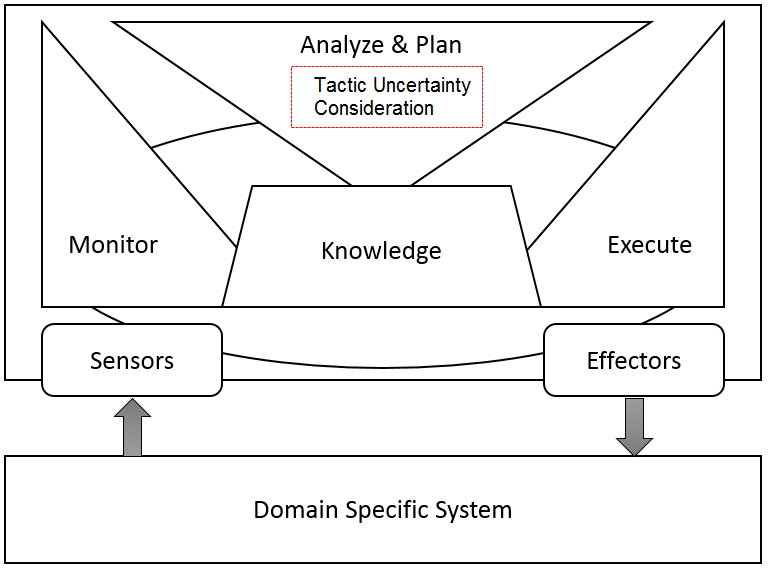
\includegraphics[scale=0.3]{images/mapek-red.png}
%      \caption{MAPE-K Self-Adaptation Loop With LVA Integrated in the `Analyze \& Plan' Stage\dan{clean up image}}
%      \label{fig:procOverview}
% %\end{wrapfigure}
%  \end{figure}
% % DK: If space is an issue, have the text wrap around the image



%%%%%%%%%




%\subsection*{Task \#1: Define Formal Framework - Adaptation Loops} % DK: Give this a different namef
%%% DK: Is this really even a task?


\section{Motivating Examples} 
We will describe two motivating examples to demonstrate the need for accounting for tactic volatility.

\vspace{3mm} \noindent \textbf{Tactic Latency Volatility} To demonstrate the need for accounting for tactic volatility during the decision-making process, we will describe a motivating UAV example. In this scenario, a UAV is searching for a missing person. The UAV's goal is to take hi-resolution photos of the area once the missing person is potentially identified. When the UAV identities the possible target, there are several steps that must be taken. In this example, the UAV's tracking camera and communications protocol with the base station requires a total time of .2 seconds to prepare and complete. This anticipated latency time means that the UAV should plan on beginning the photography process .2 seconds before it is in range. However, in the event of poor weather conditions or communication lag, it could take .4 seconds to prepare the tracking camera and perform necessary communications with the base station. Not accounting for this latency volatility could lead to a less than optimal decision, one where the UAV was past the area it wanted to photograph when the camera becomes ready for use. If the UAV was able to use knowledge about its prior mission experiences about lag with communicating with the base station, it would be better able to account for this expected lag in its future decisions. By enabling the UAV to account for tactic latency volatility and include this in its decision-making process, the UAV will be able to make a more informed decision likely enabling it to complete all mission objectives more successfully. This example scenario is shown in Figure~\ref{fig:UAVLatencyExampleCamera}. 

% ? DK: Don't make it too complicated
% In the diagram, show the UAV having a sensor to sense possible missing person to get the camera ready


\begin{figure}[h]
	\centering
    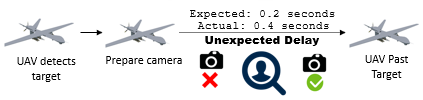
\includegraphics[scale=0.9]{images/UAVLatencyExampleCamera.png}
    \caption{Impact of Unexpected Latency in UAV}
    \label{fig:UAVLatencyExampleCamera}
\end{figure}

\vspace{3mm} \noindent \textbf{Tactic Availability Volatility} Tactics may have different amounts of availability, which should be accounted for in the self-adaptive process. In a self-adaptive system with multiple options, the system may not always be aware of the availability of each option. For example, perhaps a tactic using a remote computer is only accessible 80\% of the time, but the only way to determine this is to try the tactic. The unavailability of this tactic needs to be factored into the determination process since trying unavailable tactics will likely incur resource costs. A cloud-based system may need to interact with remote computers to retrieve required information. Due to various reasons, the connection to these remote resources may be periodically unavailable. This could be caused by network congestion, the availability of the remote server, or even cyberattacks. Regardless of how well this potential unavailability is planned for at the inception of the self-adaptive system, the system should be able to learn from previous cases of unavailability and account for this in the adaptive process. Not being able to account for this unavailability could lead to the system attempting to access these remote resources even though a similar, more dependable resource may be available. 

% \begin{wrapfigure}{r}{0.5\textwidth}
% \vspace{-10pt}
%            \centering                
%            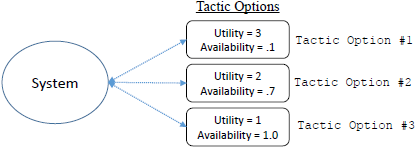
\includegraphics[scale=0.7]{images/CloudAvailabilityExample.png}
%      \caption{Impact of Availability Uncertainty}
%      \label{fig:CloudUnavailabilityExample}
%                 \vspace{-42pt}    
% \end{wrapfigure}


% DK: Does this need to be made more clearly
\begin{figure}[h]
	\centering
    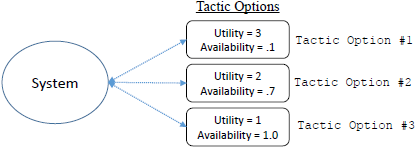
\includegraphics[scale=0.7]{images/CloudAvailabilityExample.png}
    \caption{Impact of Availability Uncertainty in Cloud Environment}
    \label{fig:CloudUnavailabilityExample}
\end{figure}

%\dan{Add more to this. Describe why current systems will fail}

Figure~\ref{fig:CloudUnavailabilityExample} displays a scenario where a system has three tactic options with identical costs, but with differing amounts of produced utility and previously observed levels of availability. The previously observed availability could have a significant impact on the decision-making process of the self-adaptive system. If the availability of each tactic option is the same, then the selection of the most appropriate tactic is a fairly simple decision since the one with the highest produced utility should be selected. However when the availability and utility of each available tactic differs, then this complicates the decision-making process. The system will need to determine which tactic option produces the best utility compared to availability ratio for the specific situation the system is in. To best make this decision of the most appropriate tactic, the system needs accurate availability information to base its decision upon.


\section{Overview of Planned TVA Process} 
Our proposed TVA approach will use several steps to enable the CPS to learn from prior experiences, including these in the adaptation process. A basic overview of these steps are:
\vspace{-2mm}
 \begin{enumerate}[noitemsep]
 	\item \textbf{Begin with initially defined assumptions} We will start with the initially defined values associated with each tactic. These values are already created for existing decision-making processes. This is where most self-adaptive systems stop.
 	\item \textbf{Record tactic observations} The self-adaptive layer will record all observed tactic values.
 	\item \textbf{Include tactic observations in the decision-making process} The tactic volatility aware component in the adaptation layer will include the observed tactic values into the utility decision process.
 \end{enumerate}
\vspace{-1mm}

We will include these tactic observations into the \emph{to be developed} Machine Learning model proposed in Task \#2. This TVA process will easily integrate into the `Analyze \& Plan' stage in the MAPE-K loop.

%, as shown in Figure~\ref{fig:procOverview}.


% \begin{wrapfigure}{R}{0.45\textwidth}
%  	\centering
%      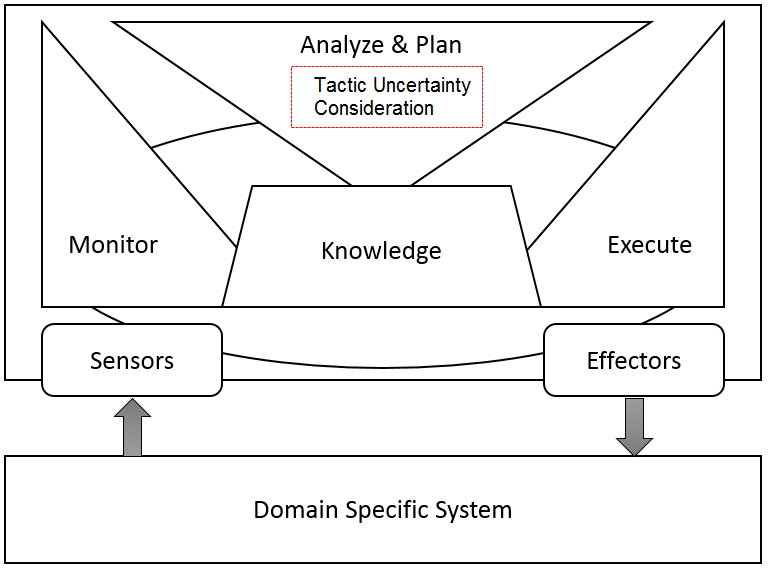
\includegraphics[scale=0.4]{images/mapek-red.png}
%      \caption{MAPE-K Self-Adaptation Loop With LVA Integrated in the `Analyze \& Plan' Stage\dan{clean up image}}
%      \label{fig:procOverview}
% \end{wrapfigure}

%% DK: Removed due to space
%  \begin{figure}[h]
%  	\centering
%      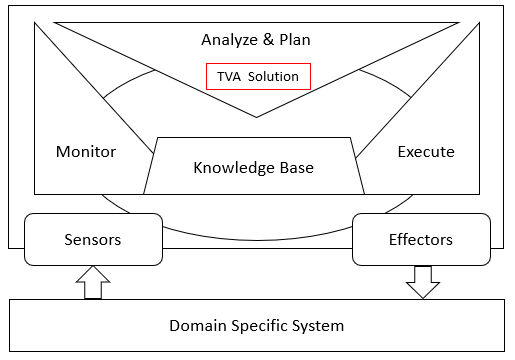
\includegraphics[scale=0.6]{images/tva-solution.png}
%      \caption{MAPE-K Self-Adaptation Loop With LVA Integrated in the `Analyze \& Plan' Stage}
%      \label{fig:procOverview}
%  \end{figure}

%%%%%%%%%%%%%%%%%%%%%%%%%%%%%%%%%%%%%%%%%%%%%%%%%%%%%
%We will develop an efficient and effective method of accounting for the tactic volatility in cyber-physical systems. By accounting for tactic volatility, we will enable the system to learn from observations; therefore reducing uncertainty and leading to more informed decisions. Although the topic of addressing uncertainty in intelligent systems has been explored, we are the first known work to focus specifically on tactic volatility. Our proposed method will be demonstrated in specific environments such as UAVs and distributed IoT systems, but will be generic enough to be applied to most adaptive decision-making processes. %Make sure what I am saying here is not redudant

%We will next describe a high-level overview of our TVA approach and how it integrates into the popular MAPE-K decision-making process that is widely used in CPS.



%%%%%%%%%%%%%%%%%%%%%%%%%%%%%%%%%%%%%%%%%%%%%%%%%%%%%%%%%%%%%%%
%%%%%%%%%%%%%%%%%%%%%%%%%%%%%%%%%%%%%%%%%%%%%%%%%%%%%%%%%%%%%%%

\subsection{Evaluation/Experimentation Plan} 
%% Required by the solicitation
%An Evaluation/Experimentation Plan that describes how proposed concepts will be validated and outlines the metrics for success;

We will systematically evaluate the effectiveness of our work in several stages, and based on several criteria. % This process is described below.


% \subsubsection*{Evaluation Process}
% \dan{Find a good simulation Process that we can use}
% %%% Evaluation process? - Should we go with iterative?
% %%		Maybe just show evolutionary approach?


\vspace{-2mm}
\subsubsection*{Evaluation Criteria}
% We will evaluate our proposed TVA process on several criteria, including: 


\begin{enumerate}[noitemsep]
%	\item \textbf{Effect on concurrent and subsequent tactic decisions:} Decisions in self-adaptive systems frequently do not occur independently of one another and may impact simultaneous or subsequent tactic decisions. Modifications to decisions-making process should not adversely affect current or subsequent tact decisions. % DK: I am not in love with this
    
  	\item \textbf{Benefit to System Resiliency:} Resiliency is a primary concern of self-adaptive systems, especially those with safety or mission-critical applications~\cite{de2014software}. We will measure the effects of TVA on the system's ability to remain resilient and complete defined objectives. %, especially when encountered unforeseen circumstances. We will also measure the system's ability to complete defined objectives, especially those that are deemed to be mission-critical.

	\item \textbf{Ability to Deal with Uncertainty:} Uncertainty comes in innumerable shapes and forms for a CPS. Some of which include component failure, cyberattacks, or even unanticipated weather conditions. A robust self-adaptive process should account for various forms of uncertainty and limit this impact on the system's resiliency, efficiency and overall effectiveness. We will evaluate the ability of our proposed TVA solution to properly account for uncertainty through several manners. We will include uncertainty mechanisms in simulators to emulate events such as software and hardware failures, along with other internal and external forms of uncertainty. 
    
   %% DK: Removed due to space
    %Uncertainty will also exist in our created, and utilized existing datasets used in our simulators. This is in addition to simulating the primary mission of our work: to account for tactic latency, availability and reliability volatility in the decision-making process. When implemented into physical devices, we will encounter uncertainty through natural means (since CPS will likely invariabliy encounter uncertainty in the wild).

% ? Give an example of how uncertainty lead to CPS failure

    \item \textbf{Lead to More Efficient Decisions:} We will measure how often the system selects the most appropriate tactic for adaptation in order to determine how efficient the decision-making process is. This will be done by counting the number of times the system selects a tactic that does not complete within its maximum allowed threshold, resulting in what we will define as a \textit{critical failure}. We will compare the results from running simulations without TVA embedded into the decision-making process, to the results from simulations where TVA is embedded into the decision-making process. 
   
    
 %   \item \textbf{Lead to Tactics with Higher Utility:} \dan{Jeff: For you}\jeff{not sure how our TVA process leads to tactics with higher utility, all we are doing is changing the decision making process, not the tactic themselves}


  	\item \textbf{Ability to be implemented into existing Self-adaptive architectures:} We will evaluate the success of this objective through the integration of our TVA process into physical devices by Co-PI Sanyal. These will include Raspberry Pis, IoT devices such as mobile ground robots with smartphones, and small UAVs. Experiments will then be conducted on these physical devices under simulated conditions, such as dropped communication links or latency in decision-making. 

\end{enumerate}

% Mention how we will compare it against baselines
% Use several different simulators (which ones) % SWIM, RUBis, IS3

\subsubsection*{Simulation Environments}
We will create and evaluate our tactic volatility based approach in several environments:

% Compare against baseline?
\begin{enumerate}[noitemsep]

%	In Full proposal should go into these steps much much more
	\item \textbf{Statistical Simulators} We will first develop and evaluate our tactic volatility aware process using statistical simulators such as $R$ and MATLAB. This evaluation will largely be used to provide initial feedback on our approach. This efficient evaluation is imperative for building our initial models and subsequently evaluating the proposed approach, including evaluations against existing techniques. These simulations will also enable efficient evaluation under different hypothetical scenarios and settings. This process will be led by Co-PI Yu.

	\item \textbf{Existing Simulation Tools} After demonstrating the effectiveness of our approach in statistical simulators, we will next perform our evaluation using existing software simulators such as RUBiS~\cite{Rubis_URL} and SWIM~\cite{SWIM_URL}. These tools emulate intelligent web systems that collect data and make adaptive decisions. We will use these tools since they are well-known, and are able to simulate numerous real-world situations. This process will be led by PI Krutz and Co-PI Yu. % We will also explore the use of other existing simulation tools as well.

	\item \textbf{Custom-Built Simulators} To provide a more robust simulation environment, we will create a custom simulation tool: \emph{Intelligent System Simulation Service} (IS3), which is further described in Task \#3. This will enable us to determine how our tactic volatility aware process works with large-scale data sets in various situations. There are several reasons for creating our own simulation tools including: I) The lack of existing options to simulate possible tactic volatility II) Existing tools do not simulate necessary events such as uncertainty to the extent required in our work III) A lack of existing datasets that contain sufficient amounts of uncertainty IV) Many existing tools are very outdated, making adoption for others challenging. PI Krutz will lead this development. % and he is experienced in creating simulation tools for intelligent decision-making systems. %\dan{Might be worth it to explain much more about these custom simulators. What will they mimic etc.....}  This process will be lead by PI Krutz and Co-PI Yu. % For the full proposal really build up this section 
           
	\item \textbf{Physical Devices} After our proposed method has demonstrated its effectiveness in several types of software simulations, we will then implement our decision-making process into several physical devices. These include single UAVs, robotic swarms, IOT devices, and a cloud-based system. Experiments will be conducted to validate the performance of decision-making with the proposed TVA approach. These experiments will be done with simulated tactic volatility situations, like dropped communication packets and latency in decision-making. This process will be led by Co-PI Sanyal.

\end{enumerate}

We will will initially use existing data sets~\cite{ita.ee.lbl.gov_URL} for our simulations, but will use our self-generated real-world data as it becomes available; especially from tests ran from our physical devices. We are well-suited to conduct this analysis due to: I) Our expertise in intelligent systems and AI II) Experience in software development III) Access to drones and other necessary physical resources. 

\subsection{Preliminary Results}
We have demonstrated the capability of our TVA approach in initial experiments. The first simulation we ran was a proof of concept in $R$, which enabled us to perform simulations that could be easily modified, and to efficiently perform regression analysis. For example, instead of running a VM to collect data about latency times and tactic decisions that could take up to several minutes to complete, $R$ performed simulations in a fraction of that time. We next used SWIM~\cite{SWIM_URL}, which simulates a self-adaptive web architecture. Therefore no modifications were needed to make the tool self-adaptive for our simulations. We used the three available tactics that are built in to the simulator for any adaptation needs, while integrating our TVA approach to aid in the decision-making process. After completing our simulations, we looked at \textit{prediction error} values, i.e. the average difference between estimated latency time and executed latency time, to determine the quantified benefit of TVA. In $R$, we saw prediction error values drop by nearly 80\% when including our TVA approach. Furthermore, our simulations in SWIM saw prediction error values drop by nearly 60\% when including our TVA approach. Although our TVA equation needs to be substantially refined and more thoroughly evaluated, this initial evaluation has demonstrated the potential for our work.

%\section{Research Description}
\section{Intellectual Merit}
This project addresses a major challenge to self-adaptive cyber-physical devices: \ul{the inability to account for tactic volatility during the self-adaptation process}. We will develop a machine learning model that leverages historical data usage of a CPS, including both the running status of its internal components and information from its surrounding environment to predict its future behavior. This will enable the system to make more informed decisions, leading to more efficient and effective outcomes while also increasing the resiliency of the system. Our TVA process will work with existing popular adaptation loops, meaning that no changes to the overall architecture of existing adaptive systems will be required. TVA will be developed and evaluated in several environments, including in actual CPSs such as drones and IoT devices. This will enable us to demonstrate the benefits of our proposed process in actual devices. The project management team possess the necessary skills (self-adaptive systems, machine learning, physical systems) to conduct all project activities. Our work will be comprised of four complimentary tasks as detailed below. 

%\dan{Amit and Qi: Can you proofread this?}

%%%%%%%%



% \begin{figure}[h] %h for here, t for top, b for bottom

% \begin{center}
% % Define block styles
% \tikzstyle{line} = [draw, -latex']

% \tikzstyle{action} = [draw=none, ellipse,fill=white!20, node distance=1.6cm, minimum height=2em, align=center]
% \tikzstyle{block} = [rectangle, draw, fill=white!20, node distance=1.6cm, text width=5em, text centered, rounded corners, minimum height=4em, align=center]
% \begin{tikzpicture}[node distance = 2.0cm, auto]

%     % Place nodes
% 	\node [block] (A) {Define Formal Framework}; % Define Formal Framework Adaptation Loops
% 	\node [block, right=1.0cm of A] (B) {CPS Implementation};
% 	\node [block,  right=1.0cm of B] (C) {Create Machine Learning Model};
%     \node [block,  right=1.0cm of C] (D) {Create Simulation Tool};
% %    \node [block,  right=1.0cm of D] (E) {Education Plan}; %DK: Include this?
	
       
% 	\draw[->] [thick] (A) to  node {} (B);
%     \draw[->] [thick] (B) to  node {} (C);
%    	\draw[->] [thick] (C) to  node {} (D);


% % - Define Formal Framework Adaptation Loops
% % - Implement into CPS
% % - Create Machine Learning Model
% % - Create IS3 Tool
% % - ? Educational Plan ?
	
% \end{tikzpicture}
% \caption{Research Plan\dan{Clean up image}}
% \label{fig:researchPlan}
% \end{center}
% \end{figure}





\subsection*{Task \#1: Controls Implementation in the Physical System}
Volatility, such as latency in tactics can lead to time delays in the feedback control loop for an autonomous system. Time delays in linear and nonlinear control systems are known to adversely impact performance and stability~\cite{Chunodkar, Samiei, Gu, Samiei2012, ebsp15}. While decision-making will be conducted by the higher level algorithms described in Task \#2 and \#3, time delays originating from latency will be accounted for in delay-independent control schemes to be created for example applications being considered here, specifically unmanned aerial vehicles (UAVs) and autonomous cars. This will vastly generalize and improve upon prior work that extends nonlinearly stable time-delayed systems that are fully actuated~\cite{Samiei2012, ebsp15}, to underactuated unmanned aerial vehicles (UAVs) and autonomous surface vehicles like autonomous cars. Underactuation is an important aspect to be considered in physical systems, where the number of degrees of freedom describing the system is more than the number of actuators (and hence control inputs) that influence these degrees of freedom. Note that most autonomous cars, and fixed-wing and rotorcraft UAVs are underactuated, with fewer control inputs than degrees of freedom of translational and rotational motion. Further, the translational and rotational motion of UAVs and autonomous cars are coupled through the control inputs. The steering control inputs fully actuate the rotational degrees of freedom, and thereby enable complete three-dimensional or planar motion, even though some translational degrees of freedom are not actuated. Nonlinear control methods for  underactuated mechanical systems that ensure stability of the system, are given in, e.g.,~\cite{bullo2004geometric,khalil:2002:nonlinear}. 


 \begin{figure}
 	\centering
     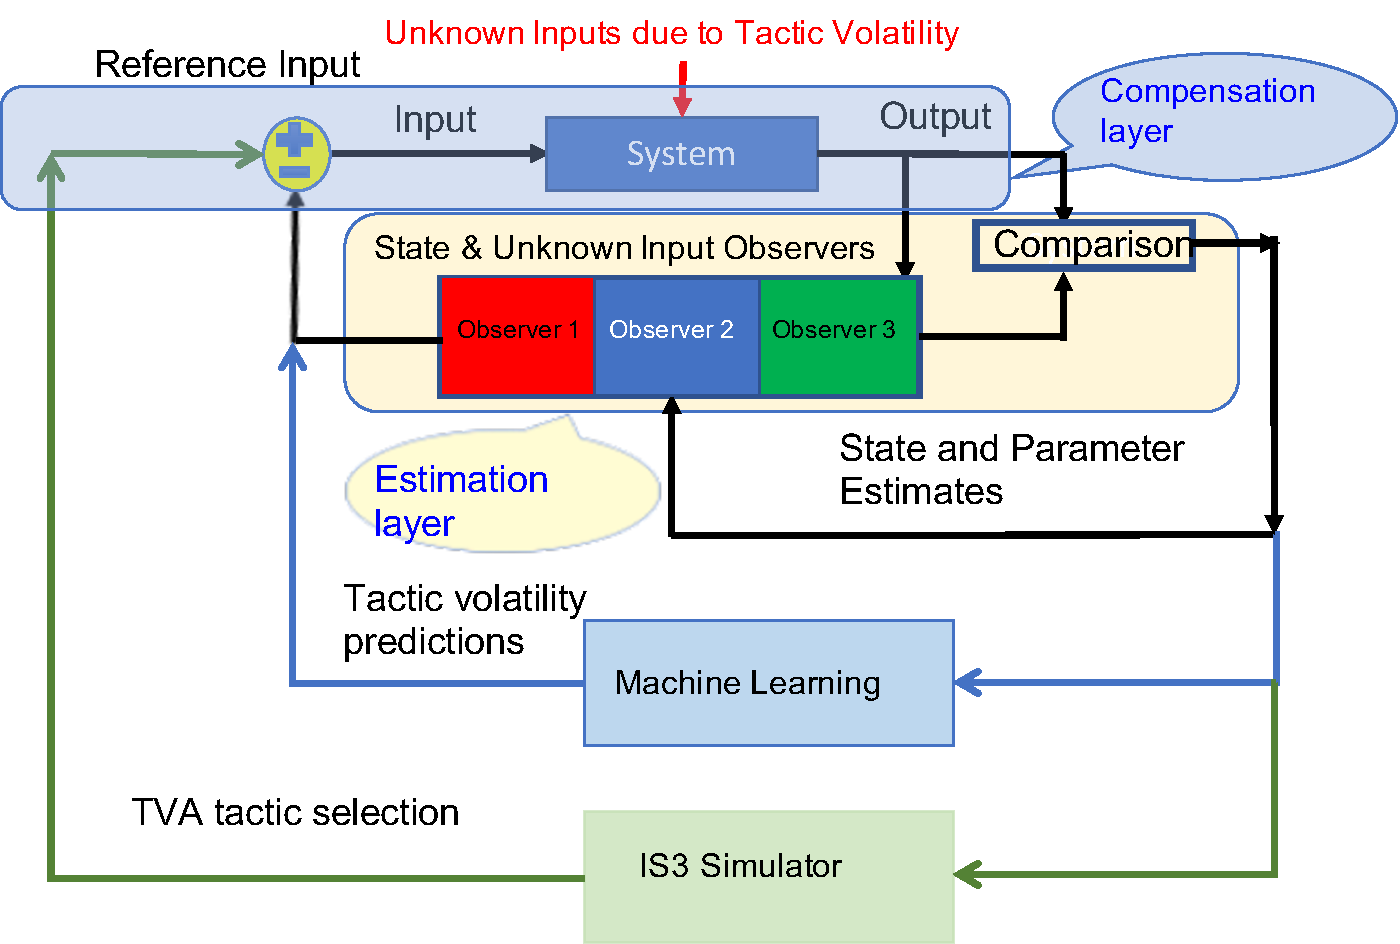
\includegraphics[scale=0.5]{images/tva_control.pdf}
     \caption{Feedback Control Using Proposed TVA Approach.}
     \label{fig:feedbackControl}
 \end{figure}



% % \begin{wrapfigure}{r}{0.4\textwidth}
% \begin{wrapfigure}{r}{0.5\textwidth}
% \vspace{-10pt}
%            \centering                
%            %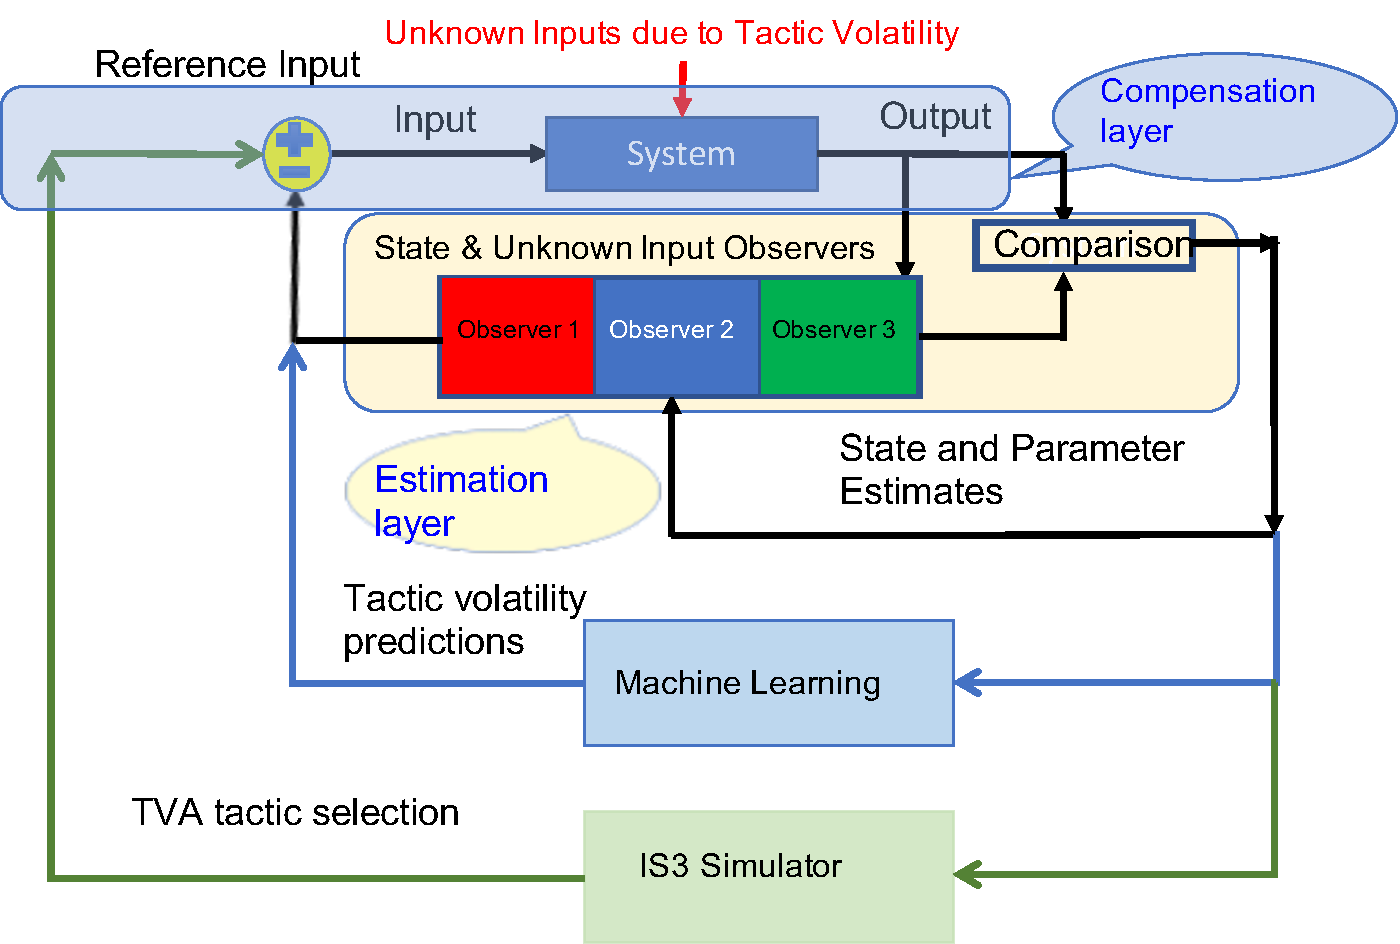
\includegraphics[width=0.30\textwidth]{images/tva_control.pdf}
%            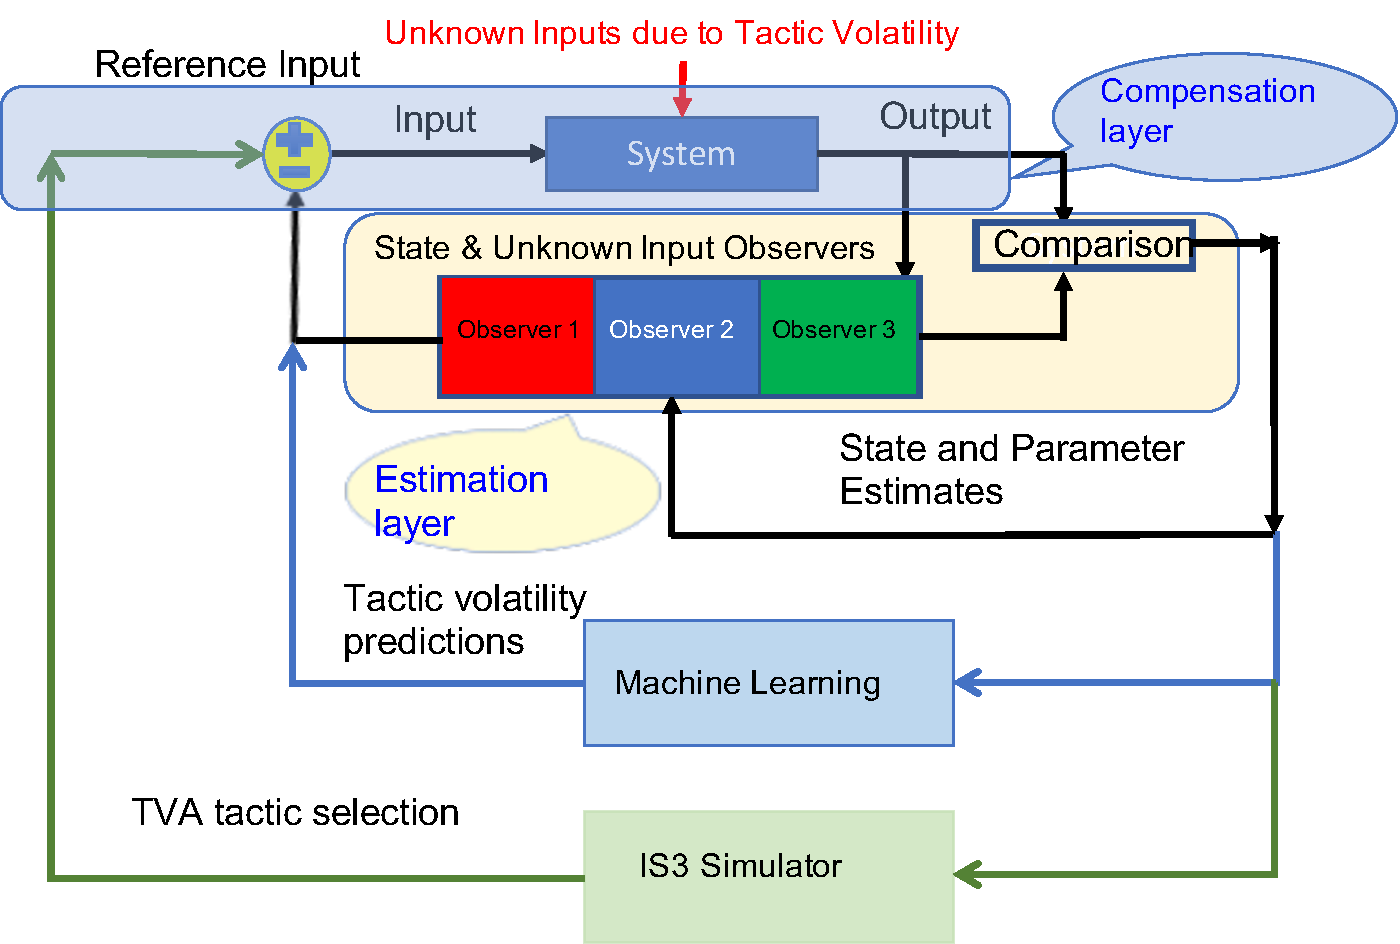
\includegraphics[scale=0.35]{images/tva_control.pdf}
%                 \vspace*{-21pt}
%                 \caption{Feedback control using TVA approach}
%                 \vspace{-12pt}
%                 \label{fig:feedbackControl}
% \end{wrapfigure}


To provide resilient control in the presence of volatility in decision-making or communications by a ground control station or human operator, the control architecture will be developed in two layers. The first layer will be the {\bf estimation layer} of the feedback control loop, which will estimate states and unknown parameters that affect the evolution time of the physical system. Internal states of the system can often be estimated without knowledge of the dynamics model of the system. For example, inertial and exteroceptive sensors can be used to estimate the states of a mobile robot without knowledge of its dynamics model using model-free nonlinear observers~\cite{auto14,relmoSE3cdc15,auto16}. However, unknown parameters that affect the operation of the feedback control system, such as time delays due to latency in decision making, and disturbance forces/torques due to changes in the environment (e.g., wind speed and weather effects on an UAV), are more difficult to measure and anticipate. Despite this, it helps us that the response of internal states to such unanticipated changes in parameters follow a predictable pattern. For example, the aerodynamic drag force on an UAV due to wind velocity is along the direction of this velocity. For this reason, estimates of states and parameters can be used by a Machine Learning model to construct better knowledge of the effects of such unknown and unanticipated parameters. A bank of observers can work in a series to complete such parameter identification tasks, as shown in Figure \ref{fig:feedbackControl}. The state estimation process is inherently robust to latency, since it uses sensors on the physical system. It also does not require a dynamics (time evolution) model of the physical system, as long as the relations between internal states and sensor measurements are known. For example, if $(\hat{x}, \hat{\theta})$ denote state and parameter estimates respectively, we will create an observer based on a Lyapunov function $\mathcal{V}_{\bar\theta}\big(\hat{x}-x(y)\big)$ for the state estimate $\hat x$, where $x (y)$ is the state as measured by the sensor outputs denoted $y$, and $\bar{\theta})$ is a known estimate of the unknown parameters. Thereafter, a second observer will be designed for $\bar\theta$ based on another Lyapunov function $\mathcal{V}_{\hat x}\big(\hat\theta-\bar\theta\big)$ that will be based on the expected dynamics of the state $\hat x$ given the parameter $\bar\theta$. The objectives of these observer designs will be to ensure that $\hat x \to x(y)$ and $\hat\theta \to\bar\theta$ in forward time~\cite{relmoSE3cdc15, miss16}. State and parameter estimates from the estimation layer will be passed on to the machine learning model of Task \#2. From historical usage data, machine learning can predict the effects of unknown inputs on the physical system, which can be used for compensation in the compensation layer of the feedback control process. This can be used to learn the effects of the parameters so that $\hat\theta\to\theta$ in forward time, where $\theta$ is the actual set of unknown parameters influencing the time evolution of the states $x(y)$.   

The second layer in the control architecture will be the {\bf compensation layer} of the feedback control loop. This layer will use state estimates from the estimation layer and unknown parameter estimates from the machine learning model, along with reference inputs that can come from a human operator or a simulation engine, to create corrective control action on the system. In our proposed approach, the tactic volatility aware selection of tactic will come from Task \#3. This will then be used to generate the reference inputs (high level tactic decisions) for the CPS. Based on the tactic chosen, the reference input is selected from a bank of possible modes of operation (e.g., nominal, aggressive, safe, etc). The physical system then follows this desired mode of operation until a tactic volatility situation requires a change in this mode. For example, a nonlinearly stable compensator can be designed to operate in mode $\jmath$, based on a Lyapunov-Krasovskii (L-K) functional $V(\hat x,t_d,\jmath)$, where $t_d$ is an assumed upper bound on the time delay due to tactic volatility. This L-K functional will be used to create a delay-independent control scheme that will compensate for the unknown time delay with the upper bound $t_d$. If the state $x$ is in a manifold $M$ instead of $\mathbb{R}^n$, as is true for UAVs and UUVs, we will use Morse-Lyapunov-Krasovskii functionals for nonlinear stability analysis in the presence of bounded time delay~\cite{ebsp15, nbys16}. This will provide robustness to time delays and external disturbances like wind gusts on an UAV. Inputs from the algorithms developed in Tasks \#2 and \#3 will provide additional information on uncertainties due to tactic volatility, while the bank of observers designed in the estimation layer will provide information on uncertain parameters affecting the real-time performance of the system. This task will be led by Co-PI Sanyal.

%\dan{I believe that a primary reason for making this task \#1 is to provide Qi's Machine learning model with data? If so, this should be mentioned in this task. Otherwise, we should perhaps move this task down}
%\amit{I responded to your emails on this, and we agree that controls and machine learning should function in an overall loop.}



\subsection*{Task \#2: Create Machine Learning Model for Accounting for Tactic Volatility}

We will develop a machine learning based prediction model to automatically and precisely quantify the tactic volatility in multiple key aspects including latency, dependability, and availability. By learning from the historical usage data of a CPS that covers both the characteristics of its internal components and control algorithms as well as features from the surrounding environment, the prediction model can anticipate the CPS's behavior in the near future. However, building such a machine learning prediction model faces several significant challenges. While various kinds of data can be collected through different channels, such as the the feedback from a feedback control scheme, onboard sensors from mobile robots (autonomous cars or UAVs or UUVs), and a ground station that is in communications with UAVs deployed in a field. There may be other {\em latent} factors that also affect the behavior of a CPS. These factors may be related to the internal running status of the CPS or something unexpected from the surrounding environment. They are referred to as {\em latent} because it is usually difficult to directly measure their values and the number of these factors also remain unknown. These latent factors may also change over the time along with running status of the CPS and its surrounding environment. Therefore, it important to systematically capture these changes and their impact on the CPS's behavior. Additionally, since latency, dependability, and availability are interrelated and correlated, instead of building three separate prediction models, it may be beneficial to construct a joint prediction model that can collectively predict all three parameters. A joint prediction model can help discover the dependency among thees parameters besides making a more accurate prediction of their values. 

We will develop a {\bf Bayesian dynamic matrix factorization model that jointly predicts multiple correlated volatility parameters}, including latency, dependability, and availability. The joint prediction model assumes that there are a number of common factors, including both observable and latent, that affect these parameters. However, they may play a different role over different parameters. We will begin by modeling the latent factors and their contribution to the parameter of interest. We will use latency as an example to derive its prediction model.  

\vspace{-2mm}\paragraph{Modeling Temporal Dynamics} Given multiple sequences of time series data for a CPS that record the latency values along with the measurable features, we represent the set of latent factors in a given sequence as a vector ${\bf f}_u \in \mathbb{R}^K$ and use another vector ${\bf l}_u \in \mathbb{R}^K$ to denote the weight coefficients of these factors to the latency parameter. The number of latent features $K$ is potentially infinite and can be automatically determined by the model. To capture temporal dynamics, we propose a state-space model to capture the latent factors that evolve with time as well as sudden changes that are not directly related to the prior running status of the CPS and the previous state of its surrounding environment. In particular, the evolution of the latent factors is modeled using the first-order Markov structure. For a given time period $t$, we have $f_{uk}^1 \sim \mathcal{N}(0,\zeta), \quad f_{uk}^t \sim \mathcal{N}(f_{uk}^{t-1},\eta)$.
To capture the time-specific changes of the latent factors, we introduce a bias term at a specific time $t$: $b_u^t \sim \mathcal{N}(0,\rho)$.
% \begin{align}
% b_u^t \sim \mathcal{N}(0,\rho)
% \end{align}
For a given sequence, since the environment and the task for the CPS is typically fixed, we assume the weights of the latent factors remain stable over time and the dynamics of the latency is introduced through the changes of the latent factors. To accommodate the uncertainty in the number of latent factors, we place an nonparametric Indian Buffet Process (IBP)~\cite{ghahramani2006infinite} prior over 
${\bf l}_u$: ${\bf l}_u \sim IBP(a)$,
% \begin{align}
% {\bf l}_u \sim IBP(a)
% \end{align}
where $a$ is the concentration parameters that control the size of the latent factors (i.e., $K$) and it can be automatically determined by the data through posterior inference. We use a vector ${\bf x}_u \in \mathbb{R}^D$ to denote the set of observable features and ${\bf w}_u \in \mathbb{R}^D$ to denote their weights. We place a Gaussian prior over ${\bf w}$: ${\bf w}_u \sim \mathcal{N} (0,A^{-1})$, where $A=diag(\alpha)$.
% \begin{align}
% {\bf w}_u \sim \mathcal{N} (0,A^{-1}), \quad A=diag(\alpha)
% \end{align}
By integrating impacts from both the latent and observable factors, a latency value at time $t$ is a drawn from the following distribution: $y^t_u \sim \mathcal{N}(\sum_k l^t_{uk} f_{uk}^t+\sum_d x_{ud}^tw_{ud}+b_u^t,\sigma)$.
% \begin{align}
% y^t_u \sim \mathcal{N}(\sum_k l^t_{uk} f_{uk}^t+\sum_d x_{ud}^tw_{ud}+b_u^t,\sigma)
% \end{align}

\vspace{-2mm}\paragraph{Modeling Infinite-dimensional Latent Factors} IBP is a stochastic process defining a probability distribution over a sparse binary matrix with an unbounded number of features. In our case, IBP is suitable as a prior for representing latent factors' weights because given a limited number of observed latency values, a small number of latent factors may actually play a role in affecting the latency of the CPS. If a large set of latency values are collected, more latent factors may be needed to cover the more diverse situations. IBP allows the model to automatically adjust its capacity based on the size of the observed data. 

The generative process of IBP can be described as follows: Consider $U$ customers who arrive at a buffet restaurant sequentially. The first customer chooses Poisson($a$) dishes, and the $u$-th customer chooses a dish with probability $n_k/u$ where $n_k$ is the number of people who have chosen the $k$-th dish previously, then chooses Poisson($a/N$) new dishes. If we represent the choices of each customer as a binary vector (1 for dishes chosen, 0 for others), the matrix constitutes a draw from IBP. This distribution is exchangeable because the order of customers enter the restaurant has no influence on the distribution. An IBP prior is assumed for matrix $L=\{ {\bf l}_u \}$. Matrix $F=\{{\bf f}_u \}$ is assumed to have potentially infinite features. However, only finite factors will interact with non-zero elements of $L$, and we only consider those factors.

\vspace{-3mm}\paragraph{Inference and Prediction} For the proposed model, it is not analytically tractable to compute the posterior distribution, because the form of posterior distribution is highly complex. In such situations, we resort to approximation schemes. Stochastic techniques such as Gibbs sampling have been implemented to construct a sample-based representation of the posterior distribution. Consider a joint distribution $p(Z |X ) = p(z_1, ..., z_k|X)$ from which we wish to sample and suppose that we have chosen some initial state for the Markov chain. At each step, we update the value of one of the variables by a draw from the posterior distribution of that variable conditioned on the values of all other variables. Then we iteratively update all variables until convergence. In our case, we can derive the conditional distribution from IBP. We first consider a case with finite latent variables, then extend it to the infinite case by taking the limit. With $K$ finite latent variables, each weight coefficient follows a Bernoulli distribution with a prior Beta distribution,
\begin{align}
p(l_{uk}|\pi_k) \sim Bernoulli(\pi_k), \quad p(\pi_{uk}|a) \sim Beta(\frac{a}{K}, 1)
\end{align}
By integrating over $\pi_k$, we have 
\begin{align}
p(l_{uk}|{\bf l}_{-uk}) = \frac{n_{uk}+a/K}{N+ a/K}
\end{align}
where ${\bf l}_{-uk}$ denotes all weight coefficients except for $l_{uk}$. We then consider a case with infinite latent variables. Since IBP is exchangeable, we can always choose an ordering such that the variable to be updated corresponds to the last customer. The last customer chooses existing dishes with probability $p(l_{uk}|{\bf l}_{-uk}) = \frac{n_{uk}}{N}$.
% \begin{align}
% p(l_{uk}|{\bf l}_{-uk}) = \frac{n_{uk}}{N}
% \end{align}
In our case this is to select any existing latent factor such that the count of that factor $n_{uk}$ is not zero. Then we also sample for new dishes for the last customer, $p(l_{uk}|{\bf l}_{-uk}) = Poisson(a/N)$.
% \begin{align}
% p(l_{uk}|{\bf l}_{-uk}) = Poisson(a/N)
% \end{align}
Therefore, the sampling scheme for prior is summarized as follows. For each sequence and existing latent factors with $n_{uk} > 0$, we set $l_{uk} = 1$ with probability given by the equation above. Meanwhile, we may add a new latent factor with probability Poisson($a/N$). After sufficient iterations, the resulting matrix will represent a draw from the distribution $p(l_{uk})$. 

To sample the full conditional distribution, we incorporate the likelihood term when sampling $l_{uk}$ for existing attributes and drawing the new attributes from a prior distribution which is Poisson($a/N$). After posterior inference, the prediction of latency at time period $T$ is given by
\begin{align}
\hat{y}^T_{u} = \mathbb{E}[b^{T-1}_u]+ \sum_k\mathbb{E}[l_{uk}]\mathbb{E}[f_{uk}^{T-1}] + \sum_d x_{ud}^{T-1}\mathbb{E}[w_{ud}]
\end{align}
where $\mathbb{E}[\cdot]$ is the expectation of a random variable. 

While we use latency as an example to derive the above modeling mechanism, it should be noted that the latent factors are jointly learned by simultaneously considering all three parameters. So, the predictions over latency, dependability, and availability are conducted collectively by the a single joint prediction model instead of three independent prediction models. Therefore, the proposed model falls into the general category of multi-task learning (MLK)~\cite{zhang2017survey}. While MLK has been intensively studied in the AI/machine learning communities, limited effort has been devoted to developing MLK models to analyze time-series data with a few exceptions (e.g., \cite{wang2012high}). Besides simultaneously modeling multiple time-series sequences, the proposed model also makes two novel contributions. First, it collectively models both observed and latent features. This {\em hybrid model} best fits the special characteristics of a CPS as not all the features that affect its running behavior can be directly observed or measured. Second, an IBP prior is adopted to automatically infer the optimal number of latent features. Such a nonparametric prior is most suitable to deal with the dynamic running behavior and surrounding environment of a CPS as the size of the latent feature space may change dynamically over time. The proposed machine learning model will be evaluated using both public datasets and the simulation environments used, and to be developed by this project. Since tactic volatility parameters (e.g., latency, dependability, and availability) take real values, the prediction model essentially conduct regression analysis. Therefore, we will adopt Root Mean Square Error (RMSE) as the major evaluation metric. The development and evaluation of our machine learning model will be led by Co-PI Yu.


%can model the following important characteristics: 1) one item only possess finite attributes, which is a small portion of the pool of attributes, while the total number of attributes is unbounded. 2) A few attributes are enough to describe a small set of items, while more attributes are required to describe a large set of items.
%Furthermore, the proposed machine learning model offers two additional major advantages that are both instrumental to gain a deeper understanding of the CPS and help choose tactics that can achieve the highest expected utility by systematically accounting for the uncertainty in the prediction that is introduced by various internal and external factors of the CPS. 



%We assume that the conditional distribution for latency $t$ is Gaussian, $p(t|x,w,\beta)=\mathcal{N} (t|w^T {\phi}(x),\beta^{-1})$, where $\phi(x)$ is the feature vector of API $x$, $w$ is the set of coefficients, and $\beta$ is the precision of the Gaussian. The feature vector is comprised of both status of internal component of the CPS as well as data collected from the surrounding environment. 
%Then, the likelihood of the training data $X$, which represents the set of historical usage of the CPS, is given by the product of the use count distribution of each usage in the set. We further assume a conjugate Gaussian prior on the weight $w$:  $p(w|\alpha)=\mathcal{N} (0,A^{-1})$, where $A=diag(\alpha).$
%Since the posterior distribution of $w$ is proportion to the product of the likelihood and prior, it is also a Gaussian due to conjugacy. Given the optimal values of $\alpha^{*}$, $\beta^{*}$, we can derive the predictive distribution over a test case $x_t$ by integrating out $w$. Besides using the mean of the predictive distribution to predict the future latency of $x_t$, the variance of the predictive distribution also provides important information to quantify the confidence level of the prediction. 

%that the mode of Gaussian distribution equals to its mean. Using the mean from \eqref{eq7} to predict target value of $x_t$ is similar to MAP. However, the Bayesian model has the advantage to quantify the certainty level of the prediction using variance from \eqref{eq7}. 

%\paragraph{Learning Process}
%\vspace{-4mm}\paragraph{Estimating parameters.} 
%Estimating hyper-parameters $\alpha,\beta$ yields a type-2 maximum likelihood problem. Specifically, we maximize the log of the model evidence given by $\ln  p(\textbf{t}|X,\alpha,\beta)  =\ln \int{p(\textbf{t}|X,w,\beta)p(w|\alpha)d w}$ where $\textbf{t} = (t_1,...t_N)^T$. By setting the partial derivative of the log model evidence with respect to  $\alpha$ and $\beta$ to zero, we compute both hyper-parameters. Furthermore, during the learning process, some $\alpha_i$ (i.e., precision of coefficient $w_i$) approaches to infinity. As a result, the corresponding $w_i$ will be driven to its mean (i.e., 0). This will result in the removal of the corresponding feature from the model, which achieves feature selection. 



\subsection*{Task \#3: Create Tool: Intelligent System Simulation Service}
%\section{Created Tool: Intelligent System Simulation Service} % Move this
We will develop a hosted, web-based simulator that will evaluate our solution in several simulated settings. The \emph{Intelligent System Simulation Service} (IS3) will fill an important need for both our project and the research being performed by others.

Developers and researchers are limited by the availability of existing and robust simulation tools to aide in the evaluation of decision-making mechanisms. While there are several simulation tools available~\cite{SWIM_URL, OMNet_URL, Rubis_URL}, they I) Do not consider real-world events such as uncertainty II) Do not simulate multiple environments/domains (cloud-based infrastructures, IoT devices and UAVs) III) Are typically not easily extensible IV) Are difficult to install and use. This lack of existing, easy to adopt, robust simulation tools not only makes the evaluation of potential decision-making mechanisms much more difficult, but can also lead to inaccurate findings due to the `one-off' nature of self-created simulation tools. Additionally, using simulation tools that do not accurately represent real world events, such as uncertainty, can lead to inaccurate/incorrect conclusions.


%More so, if existing simulation tools that do not accurately represent real-world events such as uncertainty are used, then the user may come to inaccurate/incorrect conclusions.

To address these limitations, we will develop a publicly available, hosted simulation environment referred to as \emph{Intelligent System Simulation Service} (IS3). This tool will enable researchers and developers to: I) Easily evaluate alterations to self-adaptation decision-making processes II) Understand how uncertainty will affect different adaptation systems in different settings. When analyzing a dataset, IS3 will store each set of latencies with their respective tactics. Each tactic will be run against both our TVA solution and the existing baseline equation. The system will select the tactic which was estimated to return the highest level of utility and then run the successful tactic again to verify that it made the correct decision. The result of this will be saved and used to help improve future simulations. This tool will also include public APIs for researchers to integrate into their own simulators and research tools. These APIs will emulate numerous uncertainty and security intrusions. Simulating uncertainty is important since it is typically very difficult to simulate in self-created tools.

% Get rid of redundancy
IS3 will contain the following components/features:

\begin{enumerate}[noitemsep]
	\item \textbf{Simulate Different Cyber-physical Systems} There are many different types of cyber-physical systems including UAVs (individual \& robotic swarms), medical monitoring devices and process control systems. While many of the adaptation processes are identical regardless of the specific type of CPS, there are different forms of variability and considerations that should be taken into account for each specific system. For example, a UAV will typically face many more forms of weather uncertainty than the standard medical device. IS3 will simulate each of these different scenarios including relevant events of uncertainty for each type. 
    
    
    \item \textbf{Uncertainty Simulator} Uncertainty comes in innumerable shapes and forms including internal and external uncertainty~\cite{esfahani2013uncertainty}. IS3 will enable the inclusion of many different forms of uncertainty into the simulations of numerous types of decision-making processes in various settings. This will be accomplished by including real-world data from existing APIs, and through the creation of self-created simulation mechanisms. For real-world data, we will use existing data sources such as weather APIs and live latency times for global file transfers. To create simulated data, we will use a mixture of random number generators and popular data creation mechanisms such as Symbolic~\cite{king1976symbolic} and Concolic~\cite{sen2005cute} execution to build a diverse, but realistic dataset to simulate uncertainty and as many situations as possible that the CPS may encounter. While it is impossible to simulate all forms of uncertainty, the goal is for IS3 to simulate as a wide variety of uncertainty. For example, one option will be to simulate the CPS encountering a temperature reading of -2,147,483,648 and 2,147,483,647 which are the minimum and maximum integer values. Although a CPS will quite obviously never encounter a temperature this high or low, the system should account for these values for several reasons. Perhaps a sensor failure returns an invalid reading leading to one of these extreme values, or a malicious actor is able to trick the system into receiving one of these values. The system should have the ability to gracefully handle these situations. The uncertainty simulator in IS3 will allow the evaluation alterations to the self-adaptive process to include uncertainty; an important aspect of ensuring a resilient and robust adaptation process~\cite{moreno2016efficient, Moreno:2015:PSU:2786805.2786853, camara2017uncertainty, han2016handling}. 
 
    
    \item \textbf{Dataset Creation} Robust datasets are imperative for evaluating decision-making processes for effectiveness, efficiency, resiliency and robustness. Generating these datasets can often be a difficult and time-consuming task for developers. While there are existing datasets, these are limited and may restrict researchers and developers as they may not be well-suited to many real-world situations and CPS domains. For example, the popular FIFA 98~\cite{ita.ee.lbl.gov_URL} dataset does not contain the latency times each request took, rather just a log entry that the request took place. 
    
To address the shortfalls with existing datasets, we will make ours available for other researchers to use in their own work. To ensure smooth adaptation of our datasets, they will be provided in native formats to eliminate the potential problems of decompression and corruption. Our datasets will be made available in several popular formats such as JSON, CSV, and XML. These datasets may be used within our hosted, online platform eliminating the requirement for adopters to download the datasets. Unlike existing datasets, ours will continuously collect new data, enabling it to grow and evolve.


%\hl{Unlike most available datasets, which are just a snippet in time of real-world data, we will continuously harvest data and expand upon each datasets.}



%Unlike other publicly available datasets, ours will continuously collect real world data.%, keeping the dataset up to date, reliable, and more accurate.


%	\item \textbf{Educational Component} IS3 will also serve as an educational tool, enabling users to view the decisions of the simulated UAV. Using a set of pre-defined rules along with real-time actual weather information, the simulated UAV will make an infinite number of flights around the US. An example of this component is shown in Figure~\ref{fig:educationalFlying}. %DK: Removing this for space for now since it seems pretty weak
    
\begin{figure}[h]
	\centering
    \frame{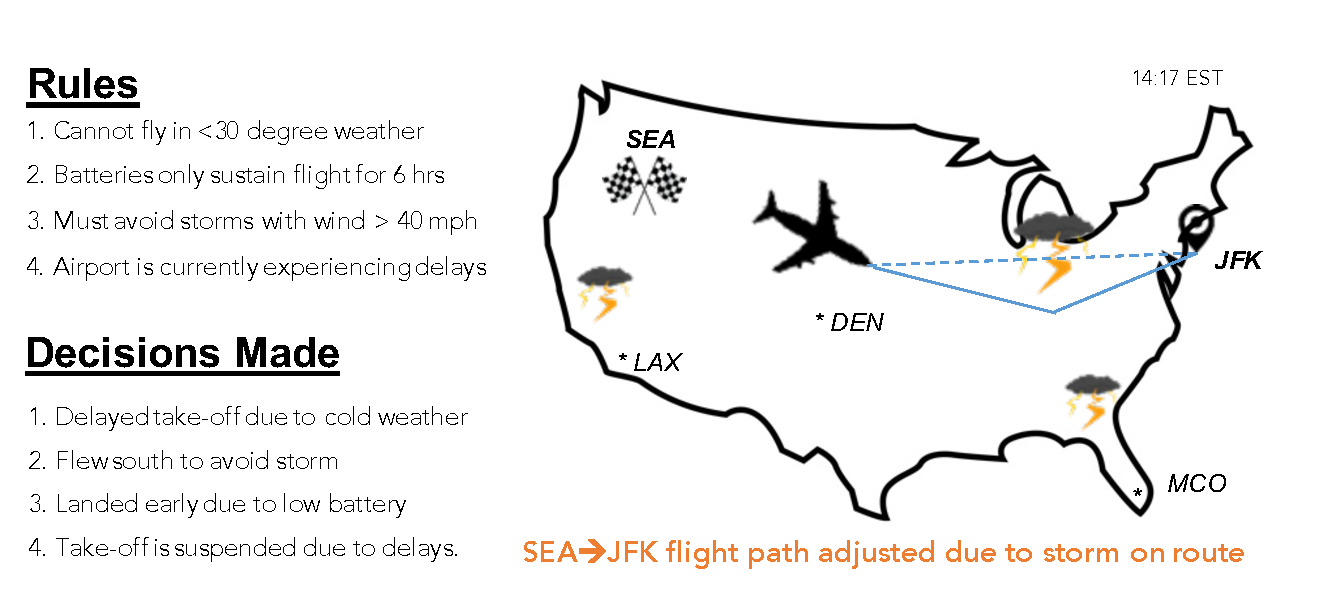
\includegraphics[scale=0.6]{images/FlightTracker-NSF.pdf}}
%    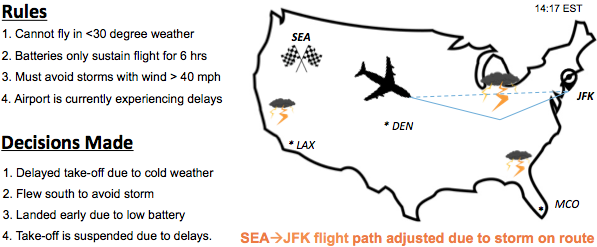
\includegraphics[scale=0.63]{images/FlightTracker-NSF.png}
    \caption{Example of IS3 Visualization Screen Showing Decision-Making Process For Simulated Airplane}
    \label{fig:educationalFlying}
\end{figure}



% DK: Show cases of uncertainty

%\dan{Stephen: Can you save as a pdf to make higher resolution. Also, clean up the text on the right and left. Also, maybe put a border around the image and make it clear that it is an output screen on the web. I know that this is tough to do in a single image, but the image needs to be largely self-explanatory. Consider making the `US' part of the image a bit larger as well as some of the items like the flag etc.... may be tough to see when printed}\stephen{Will do that now}




%% Ideas:
%	UAV flying around the US. Describe why decisions were made -> Driven by real-world data
%	Show rules on the left, map of the US in the middle and on the Right show a list of decisions-made and current system status ?

%%% Primary benefits
%	Enable students/developers to see how real-world 



\end{enumerate}




% Simulate several different settings (IoT, UAV, Swarm, etc..)
% Simulate uncertainty 
% Will contain real-world uncertainty (ping times, weather conditions etc..)
% Evaluate in terms of efficiency, resiliency, effectiveness
% Educational component
% Easy to use (hosted) - No cost or anything to install
% All source code will be publicly available
% ? Put the benefits in bullet points?
% ? What diagram can we include here?



%%%% Diagram

% ? Maybe show different screens such as updloading etc..

%\dan{I will describe our to be developed, hosted simulation tool here}


%\subsection*{IS3 System Design and Development Plan}
% Show a diagram here
% Talk about how it will be created at RIT. Will work with WiC to recruit students to create



%\dan{Should we keep this section?} % - Read the call again to make sure that it fits
% Why it is needed
% Talk about its design
% Features
% Include a screenshot here


% Will support our work, will help others
% Publicly hosted. RIT SE has a lot of experience in this area.  Resources to create and host this



% PI Krutz previously a Software Engineer in Industry, PI Krutz has a strong-track record of deliverity software projects like this in a high-quality, on time manner. Will utilize SE students. Hire WIC students. 


% Give a diagram here of how the tool will be laid out

%\subsection*{Educational Component}
% DK: Should this be moved somewhere else?






%\dan{In another section have another evaluation plan}
\newpage % Just to make things clean
Development efforts will be led by PI Krutz, who has a demonstrated record of success in creating robust, publicly available tools and datasets~\cite{krutz2013cccd, krutz2014code, krutz2015dataset, Dennis:2017:PPS:3104086.3104136, Chester:2017:MLD:3104086.3104135, McAfee:2017:CCA:3104086.3104132}. When possible, students from underrepresented groups will be hired to complete development tasks. IS3 will be an open source tool, available for public access and contributions through a GitHub project repository.


\subsection*{Task \#4: Educational Dissemination}

A primary objective of our work is to also have a direct, positive impact on CPS education. We will accomplish this by A) Conducting two camps exclusively for 8-12 grade Deaf/Hard of Hearing students to inform and motivate these students about the field of CPS and self-adaptive systems. B) Integrating elements of our research into existing curriculum at both RIT and Syracuse University.

%High School students to teach them about decision-making in CPS.

%\dan{Clean this entire paragraph up} % DK: I feel like this introduction is a bit weak
% DK: Would be good to check out other proposals to see how they word this
% 

% \hl{The educational component of this proposal will serve two functions: I) Inform students about fundamental decision-making processes inside of CPS II) Motivate students to pursue autonomous/CPS in their future academic and professional careers.}



%%%% Summer program
%	X day workshop
%	Will work with WiC, RSD (who we already have a strong relationship with)
%	

%Our work will also have a direct positive impact on the educational community. We will include all findings and the IS3 in courses that we teach. These courses include `Engineering of Self-Adaptive Software Systems' taught by PI-Krutz, \dan{Amit and Qi, and your courses here....}. The created IS3 simulation tool will prove to be especially valuable in these courses, being used to demonstrate essential course topics. All observations will be disseminated via pedagogical publications in venues such as ITiSCE, ASEE, ICSE-SEET and SIGSCE. We will also conduct at least one workshop at an educational conference such as ITiSCE (PI Krutz is on Program Committee) to share findings.


% Mention REU

 \subsubsection*{Educational Outreach Events}

We will conduct two camps exclusively for Deaf/Hard of Hearing 8-12 grade students from the Rochester area. These camps will have the primary objectives to: A) Introduce students to foundational CPS topics B) Motivate students to pursue CPS topics in their academic and possible professional careers. Each camp will be offered at no cost to approximately 24 students. These students will be recruited from the local Rochester School for the Deaf (RSD)\cite{rsd_URL}, which PI Krutz already has a close relationship with (letter of support attached). RIT has a strong infrastructure in place to support such events~\cite{RIT_KidsofCampus_URL} and has a proven track record of conducting such events. The National Technical Institute for the Deaf (NTID)\cite{ntid_url} is one of nine colleges at RIT and is the first and largest technical college in the world for Deaf/Hard-of-Hearing (Deaf/HoH) students. We will work with NTID to provide necessary accommodations to support Deaf/Hard of Hearing participants. PI-Krutz has experience conducting outreach events and working with Deaf/Hard of Hearing students~\cite{7344327}. A high-level breakdown of the daily activities are shown in Table~\ref{table:dailyEducationalbreakdown}.

\definecolor{Gray}{gray}{0.85}
\definecolor{LightGray}{gray}{0.90}

\begin{table}[h]

\begin{center}
\caption{Daily Breakdown of Educational Outreach Summer Workshop}
\label{table:dailyEducationalbreakdown}
%\begin{tabular}{| c | l |  } \hline 
\begin{tabular}{|c|L{125mm}| } \hline % use this if we want to use bullet points

  \bfseries \cellcolor{LightGray}Day & \bfseries \cellcolor{LightGray}Topics \\ \hline
%   \bfseries \cellcolor{teal!25}Week & \multicolumn{1}{|c|}{\cellcolor{teal!25}\bfseries Topic} \\ \hline

    % DK: Don't use bullet points so that we can save space
%          \begin{enumerate}[noitemsep]
%            \item Stuff
%            \item Stuff
%          \end{enumerate} 

% \begin{tabular}{L{50mm}|L{75mm} } \hline

 %  \multicolumn{3}{|c|}{XXXXX}  \\ \hline
 % \begin{tabular}{L{50mm}|L{75mm} } \hline
   %\multicolumn{2}{|L{75mm}|}{\cellcolor{Gray}\bfseries xxxx}  \\ \hline
	1 & Introduction to CPS, CPS in simulators, CPS in Raspberry PIs (hands-on) \\ \hline
    2 & Basics of self-adaptation \& adaptation challenges, CPS \& Adaptation challenges in simulators, CPS in Drones (hands-on) \\ \hline
    

% 	1 & Introduction to CPS, CPS in simulators, Project introduction \\ \hline
%     2 & Basics of self-adaptation \& adaptation challenges, CPS \& Adaptation challenges in simulators,  Project time \\ \hline


    
%    3 & Fundamentals of AI/Machine Learning Self-adaptation methods, Project time \& Initial implementation in drone netting  \\ \hline
%    4 & xxxx, Project time  \\ \hline
%    5 & xxxx, Project conclusion  \\ \hline

   \end{tabular}
  \end{center}
\end{table}


At the conclusion of the camp, participants will be given a Raspberry PI to take home. This will be pre-designed to emulate a CPS medical device, and incorporate many of the topics covered in the camp. This will enable students to continue learning even after the camp concludes. These Raspberry PI-s will be provided at no cost to camp participants. All curriculum used in the educational events along with key observations will be publicly made available on the project website, and in publications and at least one workshop in a conference such as SIGSCE, ITISCE, ASEE or FIE. PI Krutz will lead all outreach efforts. % DK: Maybe this should go into broader impacts

%%% DK: Include if we have space
%The camp will also include guest speakers from local companies and government officials who will discuss the needs of CPS professionals and pathways to these careers. PI-Krutz has an existing relationship with several speakers who have expressed a desire to speak at these camps. When possible, we will include speakers from underrepresented groups, so that they may serve as role models to participants of these groups.






%%BI
%? Will conduct a workshop at an educational conference such as ITiSCE (PI is on PC) to share findings and results. Will publish educationally-oriented paper on these findings. 



%%%%%% Activities
% Basics of self-adaptation
% Basics of CPS
% Using their Raspberry Pis
% Putting code into CPS
% Concluding project
% Flying a drone in RIT drone cage
% Public speaker series  (Could come from DOD who we have a strong relationship with - Will seek to have a speaker from an underrepresented group)
%     





\subsubsection*{Classroom Integration} % DK: I feel like this title is weak

This project will also positively impact courses being conducted in three programs spanning two universities. These include self-adaptive systems (PI-Krutz), Data-driven Knowledge Discovery (Co-PI Yu), and Nonlinear and Optimal Control (Co-Pi Sanyal). Participating PhD students will also share knowledge across the colleges. The PI of a Software Engineering REU at RIT (Dr. Mehdi Mirakhorli) has invited us to conduct technical sessions on CPS in this REU (letter of support attached).


% All results will be disseminated


%%%%%%%%%%%%%%%%%%%%%%%%%%%%%%%%%%%%%%%%%%%%
% Include in courses that we teach
% Week/end educational session for students in the Rochester/Syracuse area
% Disseminate at workshops
% Will work with WiC/NTiD/City schools to find underrepresented participants
% PhD students will share knowledge across the colleges
% Will make use of the REU at RIT
% Students can implement decisions in drone cage at RIT
% Project inside of drone cage
% Provide students Raspberry PI which will act as a CPS. Take home
% Mention how students will be recruited -- show we have a plan to get students
% 



% \section{Dissemination Plan}
% \dan{Should we include this section?}
% Our work will be disseminated in several venues related to CPS/Autonomous systems machine learning. Some of which include ICSE, FSE, AAAI and SEAMS. We will also present educational findings in venues such as SIGSCE, ITiSCE and ASSETS. We will conduct at least one workshop in each of these areas to further present our findings. \dan{add to this if we are going to keep it\dan{I will remove this section, but I am just leaving it in for now as a reminder to make sure that dissemination is sprinkled throughout the rest of the proposal}}





% Probably copy much of this from other proposals

% Workshops (CPS and educational)
% Conferance papers?





% Does the educational component go in here

% Use the simulator in outreach events
% Simulator will be presented at conferences to publicize its availability. PI-Krutz is experienced in developing and disseminating tools
% 








% An external advisory group will chaired by External Educational Howles. This group will provide external, objective feedback on the progress of the project and make recommendations necessary to improve the direction of the project. The advisory group will consist of: Richard Ladner, a Professor Emeritus in Computer Science \& Engineering at the University of Washington who is an experienced access technology researcher; Paula Brown a Professor of Speech-Language Pathology in Communication Sciences \& Disorders at Nazareth College; Kim Berry a Speech-Language Pathologist at Clarke Schools for Hearing and Speech, NY. The group will meet quarterly via conference call and provide feedback on all project materials and results. Their evaluation results will be presented to the project management team in a written report. 




% Figure~\ref{fig:xyz}

% \begin{figure}[ht!]
% \centering
% 
\includegraphics[scale=0.75]{images/dummy.png} 
%   \caption{xxxx}
%   \label{fig:xyz}
% \end{figure}


% \begin{enumerate}[noitemsep]
% 	\item xxxx
% 	\item XXXX
% \end{enumerate}


%\subsection{Intellectual Merit}
% DK: Required per solicitation




% Current and real world challenges in these systems

% TVA process will be developed and evaluated in several envrionments, including in actual CPS such as drones; allowing us to demonstrate the impact of our improvements.

% We will address real-world problems in these systems. 
% Will not create a need for other changes in the adaptation loop. Will be able to work with existing systems and structures.












\section{Broader Impacts}
% DK: Required per solicitation
% Not sure if these should be broken up by bullet points


% Broader Impacts that describe how the research outcomes, which includes Broadening Participation in Computing, will be disseminated to a wide audience, go beyond traditional academic publications, and includes education and outreach from the research team spanning multiple levels of engagement.


Achieving a broad impact on the decision-making component of CPSs is the ultimate goal of this project. We summarize our project impact in the following areas:

\begin{enumerate}[noitemsep]
\item \textbf{The project can positively impact large numbers of autonomous CPS in terms of resiliency, efficiency and effectiveness.} Cyber-physical systems will continue to become more ubiquitous, fulfilling a variety of new and different tasks. As these systems become more prevalent, the demand for better decision-making mechanisms in these systems will also grow. Our TVA process will easily integrate into existing adaptation control loops such as MAPE-K, making it adoptable by a large number of CPS and other autonomous systems. These results will be disseminated in publications and workshops at venues such as ICSE, FSE, AAAI and SEAMS.

\item \textbf{Our IS3 simulation tool will enable other researchers to utilize our publicly available, hosted simulation environment and data sets in their own work.} Our IS3 simulation tool will be the first known of its kind that enables others to A) Evaluate existing and self-created alterations to the adaptation process in simulated environment using real-world data containing real-world variability B) Provide a large, continuously growing dataset of real-world events that others may easily download and use in their own development and research C) Is hosted, enabling easy adoption. Researchers, educators, and students of CPS will be positively impacted by the creation of IS3. This tool will be disseminated in the tool track at venues such as ICSE, FSE and ASE.

%Our hosted, IS3 simulation tool will be developed in parallel with the rest of our work to ensure that it offers 

% Simulate real-world events, such as uncertainty
% Created with real-world data
% Hosted so it will be easily adoptable by others

\item \textbf{Our outreach camps will directly benefit at least 48 Deaf/Hard of Hearing students in the field of CPS and autonomous systems.} Our camps will be the first known educational workshops in CPS systems that specifically target the Deaf/Hard of Hearing population. These camps will inform students about foundational concepts in CPS using both instructional and hands-on activities with physical devices such as drones (RIT possesses a drone cage). We will disseminate all observations and created project materials in venues and workshops such as SIGSCE, ITiSCE and ASSETS.

\end{enumerate}

We will actively engage undergraduate and female students in this project. PI Krutz has a strong track record in this aspect and regularly works with the Women in Computing (WiC)\cite{wic_URL} group at RIT.

%\vspace{-8mm} % Can use this to reduce space between Project Management and Project Timeline sections
\section{Project Management and Collaboration Plan}
% DK: Required per solicitation

\noindent PI Krutz will coordinate all project activities. He is proficient in self-adaptive systems~\cite{7774954, Krutz2018SeamsTemp} and will also lead the integration of the enhanced tactic volatility aware solution into the self-adaptation loop. PI Krutz will also manage all conference workshops, and the two camps for Deaf/Hard of Hearing grade 8-12 students. He has previous collaborated with the National Technical Institute for the Deaf~\cite{7344327} and will work with them to recruit students and conduct activities for the Deaf/Hard of Hearing participants.

% PI Krutz will organize the creation of all labs. In addition to having extensive software development experience, he has experience in creating educational labs~\cite{krutz2016teaching}. PI Krutz will also manage the overall project and the inclusion of the labs in courses at RIT. PI Krutz is a first year tenure track Assistant Professor at RIT who has a long track record of including underrepresented and undergraduate students in research projects.

\vspace{3mm} \noindent Co-PI Qi Yu will be responsible for the machine learning based prediction model. He has been working in the field of machine learning and data mining for over 10 years. His work focuses on developing and leveraging machine learning models to analyze massive modern data collections generated from diverse domains. Co-PI Yu's work has resulted in over 80 publications, many of which appeared in top-tier venues. 
% Serve as the Machine learning expert, which he has a strong background in\todo{cite}


\vspace{3mm} \noindent Co-PI Amit Sanyal will be 
responsible for design and implementation of control algorithms on some physical systems. His expertise is in nonlinear control and estimation techniques, and has been active in these fields for 15 years. His research techniques and background will be particularly beneficial to this project in demonstrating the resiliency of the proposed TVA methods in CPS applications.  
%....\dan{All: Can you update these sections}
% Lead impelemtnation into physical systems

%PI Krutz CO-Pi Yu, and Co-Pi Sanyal have collaborated on previous .\dan{Ok to say this since we did submit to ASE?}  




% Team will serve to benefit one another since we are all experts into a diverse areas, that will enable us to come together to solve this critical problem .... Too corny


% Why is 1+1+1 > 3
% Complimentary skill sets
% 

% If we go the larger route, we will need to really build on the collaboration plan


% \subsection{External advisory group}
% An external advisory group will be comprised of the following individuals XXXXX (chair), XXXX, XXXXX. This group will review our progress, and initial findings; providing feedback to the project management team in a written report. The group will meet once a year in person, and every other quarter via remote meeting.
%chaired by Xxxx  Their evaluation results will be presented to the project management team in a written report. \dan{? Include this?}

% DK: Obviously finish this

% USAF
% Gabriel?
% RIT Imaging Science
% https://nuairalliance.org/about-the-nuair-alliance/
% GATech
% 




% \section{Facilities Available to Accomplish Research Objectives}

% %\begin{figure}[h]
% \begin{wrapfigure}{R}{0.45\textwidth}
%  	\centering
%      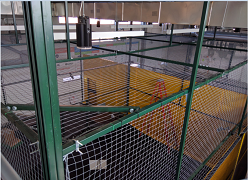
\includegraphics[scale=1.0]{images/SUFac1_sm.png}
%      \caption{UAV Cage Structure at Syracuse}
%      \label{fig:suUAVCage}
% \end{wrapfigure}
% %\end{figure}


% RIT and Syracuse University currently possess the necessary facilities to complete the proposed work. Research Computing~\cite{RIT_ResearchComputing_URL} at RIT provides high performance computing resources. They have six Sun Fire X4600 M2 servers with eight quad-core 2.3GHz AMD processors and 64GB of memory each along with two Sun Fire X4500 servers that hold 48TB of raw data each. It is operated under a shared-resource model. The Center for Advanced Systems and Engineering (CASE) at Syracuse University, has an experienced and FAA-certified UAV pilot (Mr. Ian Joyce), supercomputing facilities, rapid prototyping and microprocessor boards for onboard testing of estimation and control algorithms. Co-PI Sanyal's home lab at the Syracuse Center of Excellence (CoE), which has a 20 ft × 20 ft × 18.5 ft indoor caged-in volume that is available for safe indoor testing of UAVs (Figure~\ref{fig:suUAVCage}). This indoor UAV lab posses several lightweight quadrotor UAVs; a DJI Phantom 4 quadrotor UAV; three custom-built UAVs; several LiDAR, optical and inertial sensors; two PX4 autopilots; BLDC motors with control units; and a customized autopilot with a sensor suite and onboard processor for autonomous navigation and control. It is mounted with an eight-camera Vicon motion capture system that can be used in two modes: (1) to provide motion estimation for feedback control of UAV platforms within the caged-in volume; and (2) as an external verification and validation system for onboard observer and control schemes for trajectory and target tracking. This camera system is accessed through a high-performance desktop computer that also acts as a control station to upload waypoints and Simulink-generated target code to UAVs flying inside the cage structure. A picture of this space is given below left, alongside a picture showing a still photo of an experiment using one of the Syma quadcopters in an autonomous trajectory following maneuver, where the motion feedback was provided by the Vicon system.\dan{Amit: edit if needed}

% % DK: Cut down if space is an issue



% %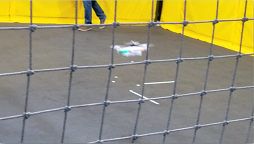
\includegraphics[scale=0.3]{images/SUFac2_sm.png} 

% % \begin{figure}%
% %     \centering
% %     \subfloat[UAV Cage Structure St Syracuse]{{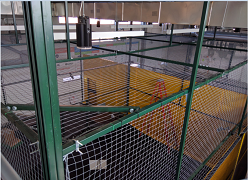
\includegraphics[scale=0.9]{images/SUFac1_sm.png} }}%
% %     \qquad
% %    \subfloat[label 2]{{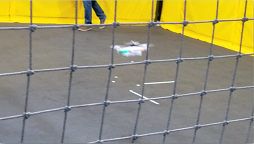
\includegraphics[scale=0.9]{images/SUFac2_sm.png} }}%
% %     \caption{2 Figures side by side}%
% %     \label{fig:Su}%
% % \end{figure}











% %RIT possesses a Guidance, Navigation and Controls (GN\&C) Laboratory and a state-of-the-art machine shop available to all students and faculty that can be used for constructing necessary any hardware as described in ``Goal XXX''. Algorithm development required for Goal X can be accomplished at RIT's GN\&C lab using currently owned algorithmic development tools such as Matlab. In addition, RIT possesses a unique outdoor netted UAV testing enclosure that can be used for final demonstration of the prototype flying UAV system. The advantage of the netted enclosure is no special FAA certificates or exemptions are required to perform outdoor demonstration testing. 





% %\dan{Add in Syracuse info}
% %\dan{Add in Griffis information}
% %\dan{Add in several photos}

% %RIT/Syracuse have the computers required for algorithmic development and demonstration tasks. We anticipate that no other capital equipment is required.



% %% Tie each into tasks

 
\section{Project Timeline}%\dan{probably just more or less tie these into tasks. Make as short as possible}


The development timeline of the project will progress as shown in Figure~\ref{fig:ProjectTimeline}.%\dan{Amit \& Qi: Add what you feel is necessary here}. 



%%%%%% Begin project timeline


% Add in TaskID and clean up the bleeding together of the cells ? Maybe a cell image?  

\newcounter{loopcntr}

\newcommand{\on}[1][1]{
  \forloop{loopcntr}{0}{\value{loopcntr}<#1}{&\cellcolor{gray}}
}
\newcommand{\off}[1][1]{
  \forloop{loopcntr}{0}{\value{loopcntr}<#1}{&}
}
 \begin{figure}[h]
 \begin{center}
 \begin{ganttchart}[
y unit title=0.5cm,
y unit chart=.6cm, %1.0 by default %<- Change this to adjust height
x unit=0.9cm, % Width
title height=1,
title label font=\bfseries\footnotesize,
hgrid, 
vgrid,
%vgrid={*4{red}, *4{blue}, *4{orange}}, 
bar label font=\small,
bar label node/.append style=%
{align=right}
]{1}{12}
%%%%%%% Start: Title (Years) %%%%%%% 
\gantttitle{Year 1}{4}
\gantttitle{Year 2}{4}
\gantttitle{Year 3}{4}  \ganttnewline
%%%%%%% End: Title (Years) %%%%%%% 
%%%%%%% Start: Subtitle (Quarters) %%%%%%% 
\gantttitle[title label font={\tiny}]{Q3}{1}
\gantttitle[title label font={\tiny}]{Q4}{1}
\gantttitle[title label font={\tiny}]{Q1}{1}
\gantttitle[title label font={\tiny}]{Q2}{1}
\gantttitle[title label font={\tiny}]{Q3}{1}
\gantttitle[title label font={\tiny}]{Q4}{1}
\gantttitle[title label font={\tiny}]{Q1}{1}
\gantttitle[title label font={\tiny}]{Q2}{1}
\gantttitle[title label font={\tiny}]{Q3}{1}
\gantttitle[title label font={\tiny}]{Q4}{1}
\gantttitle[title label font={\tiny}]{Q1}{1}
\gantttitle[title label font={\tiny}]{Q2}{1}\\
%%%%%%% End: Subtitle (Quarters) %%%%%%% 
%%%%%%% Start: Tasks %%%%%%% 

% Task 1
\ganttbar[bar/.append style={fill=black!50}]
	{Controls Implementation in the CPS}{1}{12} \ganttnewline

% Task 2
\ganttbar[bar/.append style={fill=black!50}]
	{Create Machine Learning Model}{1}{12} \ganttnewline


% Task 3
\ganttbar[bar/.append style={fill=black!50}]
	{Create IS3 Tool}{1}{12} \ganttnewline


\ganttbar[bar/.append style={fill=black!50}]
{Algorithm Development}{1}{10} \ganttnewline



%\ganttbar[bar/.append style={fill=black!50}]
%{Implementation \\ into CPS}{1}{1} \ganttnewline


%%%%% Evaluation
\ganttbar[bar/.append style={fill=black!50}]
{Evaluation}{3}{12} \ganttnewline

%\ganttbar[bar/.append style={fill=black!50}]
%{}{9}{9} 

%\ganttbar[bar/.append style={fill=black!50}]
%{}{12}{12}  \ganttnewline
%%%%%%% End: Evaluation %%%%%%% 



%%%%% Student Workshop
\ganttbar[bar/.append style={fill=black!50}]
{Student Workshop}{8}{8}

%\ganttbar[bar/.append style={fill=black!50}]
%{}{9}{9} 

\ganttbar[bar/.append style={fill=black!50}]
{}{12}{12}  \ganttnewline
%%%%%%% End: Tasks %%%%%%% 

%%%%% Conference Workshop
\ganttbar[bar/.append style={fill=black!50}]
{Conference Workshop}{8}{8}

%\ganttbar[bar/.append style={fill=black!50}]
%{}{9}{9} 

\ganttbar[bar/.append style={fill=black!50}]
{}{12}{12}  
%%%%%%% End: Tasks %%%%%%% 


\end{ganttchart}
 	\caption{Project Timeline}
     \label{fig:ProjectTimeline}
     \end{center}
\end{figure}
 
 
% Task \#1: Controls Implementation in the Physical System
% Task \#2: Create Machine Learning Model for Accounting for Tactic Volatility
% Task \#3: Create Tool: Intelligent System Simulation Service
% Task \#4: Educational Dissemination
 
 
 
% Major actions
% Implement into Physical Items
% Education outreach
% Develop and evaluate formulas
% Create IS3 tool


 
%%%%%% End project timeline

%%%%%%%%%%%%%%%%%%%%%%%%%%%%%%%%%%%%%%%%%%%%

\vspace{-8mm}
\section{Results from Prior NSF Support}

 %\noindent
 \textbf{PI Daniel Krutz} has had no prior NSF support.

 \vspace{2mm} \noindent
 \textbf{Co-PI Amit Sanyal} PI on NSF project {\em CMMI 1131643, Robust State and Uncertainty 
Estimation for Unmanned Systems in the Presence of External Uncertainties}, \$278,158, period of performance 9/2011-8/2014.  
{\em Intellectual merit}: (1) state estimation from noisy measurements with bounded noise, 
generalizing sigma-point filters to the nonlinear state space of  rigid body motions~\cite{cdc12}; 
(2) estimation of uncertain parameters for control control of rigid body 
dynamics~\cite{jgcd12,joss13,wkbs13}; (3) robustly stable estimation schemes for rigid body 
dynamics with bounded disturbance inputs~\cite{dscobs13,cdcobs13}; and (4) rigid body 
attitude control in the presence of stochastic inputs and unknown time delay~\cite{ebsp15}. 
{\em Broader Impacts}: Outreach efforts include working with the NM Alliance for Minority 
Participation (NM-AMP) and demonstrations in the PI's lab for local school students through 
southern New Mexico SEMAA. An undergraduate (Calvin Silas) supported through 
NM-AMP helped fabricate a 3D attitude control testbed and design a website for presenting 
research findings. Scholars partly supported: three Ph.D. students and one post-doctoral 
scholar.

Co-PI on NSF project {\em CNS 1739748, CPS: Medium: Enabling Multimodal Sensing, Real-time 
Onboard Detection and Adaptive Control for Fully Autonomous Unmanned Aerial Systems}, \$400,000, 
(PI: Qinru Qiu), period of performance 10/2017-9/2019. 
{\em Intellectual merit}: The primary goal is to create fast onboard waypoint allocation, trajectory 
generation and adaptive control schemes using computer vision and machine intelligence algorithms 
in GPS-denied and/or cluttered indoor environments. The unified computation model simplifies the 
hardware design, and allows for low-cost and low-power hardware, which is highly optimized for 
inference and training of deep neural networks. {\em Broader impacts}: This project will advance 
UAV technology and benefit machine intelligence and robotics communities. The proposed framework 
enables UAVs to operate autonomously in poorly known or unknown environments and in the 
absence of external navigation aids, with limited human oversight. 
 %\dan{Amit: Can you update this section}

 \vspace{2mm} \noindent
 \textbf{Co-PI Qi Yu} has had no prior NSF support.




% \pagebreak
% \dan{Not sure where to put this}
% \subsection{Preliminary Results}
% \dan{NOt sure where to move this, but I'd keep it short and just mention some of our early findings. Don't need to get too deep}
% \dan{Include this section?}\dan{Update this all with some results from the ASE paper}

% As an initial demonstration of the potential effectiveness of accounting for latency volatility during the decision-making process, we conducted several simulations to demonstrate the benefits of accounting for tactic latency volatility during the decision-making process. 





% \todo{Give an introduction to this section}



% % Add things from latency uncertainty and other simulations. Don't give too much away since we don't want to make it seem like we already did the work

% Equation~\ref{eq:proposedLVA} was created to account for latency variability when estimating tactic utility at the time of an adaptation decision. 

% \begin{equation} 
%     U = \dfrac{(T - L_A)*W}{SD_A}
%   	\label{eq:proposedLVA}
% \end{equation}

% \jeff{this needs to be updated, very old, I will take care of this}This approach considers utility ($U$) to be dependent on the adaptation decision period ($T$), the latency distribution ($L$) of the tactic being executed, and the impact of the tactic, noted as ($W$). Equation~\ref{eq:proposedLVA} accounts for tactic latency volatility by dividing the overall result in the numerator by the standard deviation of the tactic's latency distribution. This process, otherwise known as standardization, enables us to conform our utility values to a norm. By conforming the utility values to a norm, our LVA technique can not only accurately account for latency variability, but also give us resulting tactic utility values that can be appropriately compared. Therefore, any uncertainty that might exist in a tactic's latency distribution can be minimized, thus leading to more accurate adaptation decisions. 


% We evaluated the possible benefits of using our latency volatility aware formula in two different platforms I) R scripts II) In a small, custom-built simulation environment........


% \noindent\rule{12cm}{0.4pt} \\
% \dan{Update all of this with data from our ASE paper}
% \vspace{80mm}

% \noindent\rule{12cm}{0.4pt} \\


% Although these preliminary results are encouraging and demonstrate the potential benefits of accounting for tactic volatility I) This method only accounts for tactic latency volatility, not other forms of tactic volatility II) Further analysis needs to be conducted, including implementing into real-world devices and scenarios.

% Further evaluate it
% Implement into different OIOT devices
% Incorporate other forms of volatility




%\section{Research Description}












% \subsection{Technical Challenges}
% \dan{Make every section have this}
% %In this section the principal investigator answers questions such as, “What are the specific technologies to be developed?” or “What are the specific difficulties to be encountered?” It lists the technical hurdles that must be overcome to meet the technical objectives, identifying the ones that are the most important or the most difficult. This section should require one page at most. 


% There are several technical challenges that must be overcome in both development and evaluation of our proposed work.


% The first challenge to overcome is that uncertainty is difficult to plan for. Due to the inherit variable nature of uncertainty, it is challenging to incorporate into many decision-making models, and can be difficult to even test for. To address this challenge, we will use existing datasets\hl{finish....}


% % Also describe risks. Maybe look at listing them like L, M, H - Maybe steal this from AG's proposal


% \todo{Simulating battlefield situations is hard} % For the tool
% \todo{How to decide the most appropriate utility}


% % Create simulations
% % Including in actual devices
% % Uncertainty is ..... (cite some existing workds)
% % Uncertainty by its very nature is unknown



% % Where will we get our data

% Simulating uncertainty is frequently a difficult challenge

% %One is what does it mean to simulate uncertainty? Uncertainty could be because there is no way to know something because it changes all the time. In that case you’d be simulating the thing that changes. But uncertainty can also be about not knowing something that is knowable. So, how is that going to be simulated?



% % Simulation Creation



% % Physical Testing
% The final stage of evaluating and demonstrating the impact of our findings will be to incorporate our improved decision-making process into physical devices, such as drones and IOT devices. We are confident in our abilities to address these challenges due to our expertise in software engineering, and the University's extensive drone research infrastructure. % DK: Add more to this




% %\section{Educational Plan}\dan{Move this?} % DK: I am not sure exactly where this should go. 




















%%%%%%%%%%%%%%%%%%%%%%%%%%%%%%%%%%%%%%%%%%%%%%%%%%%%%%%%%%%%%%%%%%

%% http://www.splitpdf.com: Split references off of main document (Might make files that are not readible)


% Find way to only print refs document to be safer

%\pagebreak
\clearpage 

\setcounter{page}{1} % Create new page counter for bibliography
\pagenumbering{roman}

\bibliographystyle{abbrv}
%References Cited
\bibliography{refs}
\end{sloppypar}


\end{document}



%% Questions:


% Use Gab's introduction since it is good. Mimic it
% Put section about current work about uncertainty somewhere in the paper
% Might be a good idea to use something like Figure 1
% Make sure to cite this paper and add it to the related works
% ASE: Talk about how it fits into the MAPE-K loop. Where does it fit in


% We do not seek ways to 






